% Options for packages loaded elsewhere
\PassOptionsToPackage{unicode}{hyperref}
\PassOptionsToPackage{hyphens}{url}
%
\documentclass[
  ignorenonframetext,
]{beamer}
\usepackage{pgfpages}
\setbeamertemplate{caption}[numbered]
\setbeamertemplate{caption label separator}{: }
\setbeamercolor{caption name}{fg=normal text.fg}
\beamertemplatenavigationsymbolsempty
% Prevent slide breaks in the middle of a paragraph
\widowpenalties 1 10000
\raggedbottom
\setbeamertemplate{part page}{
  \centering
  \begin{beamercolorbox}[sep=16pt,center]{part title}
    \usebeamerfont{part title}\insertpart\par
  \end{beamercolorbox}
}
\setbeamertemplate{section page}{
  \centering
  \begin{beamercolorbox}[sep=12pt,center]{part title}
    \usebeamerfont{section title}\insertsection\par
  \end{beamercolorbox}
}
\setbeamertemplate{subsection page}{
  \centering
  \begin{beamercolorbox}[sep=8pt,center]{part title}
    \usebeamerfont{subsection title}\insertsubsection\par
  \end{beamercolorbox}
}
\AtBeginPart{
  \frame{\partpage}
}
\AtBeginSection{
  \ifbibliography
  \else
    \frame{\sectionpage}
  \fi
}
\AtBeginSubsection{
  \frame{\subsectionpage}
}
\usepackage{amsmath,amssymb}
\usepackage{iftex}
\ifPDFTeX
  \usepackage[T1]{fontenc}
  \usepackage[utf8]{inputenc}
  \usepackage{textcomp} % provide euro and other symbols
\else % if luatex or xetex
  \usepackage{unicode-math} % this also loads fontspec
  \defaultfontfeatures{Scale=MatchLowercase}
  \defaultfontfeatures[\rmfamily]{Ligatures=TeX,Scale=1}
\fi
\usepackage{lmodern}
\usetheme[]{CambridgeUS}
\ifPDFTeX\else
  % xetex/luatex font selection
\fi
% Use upquote if available, for straight quotes in verbatim environments
\IfFileExists{upquote.sty}{\usepackage{upquote}}{}
\IfFileExists{microtype.sty}{% use microtype if available
  \usepackage[]{microtype}
  \UseMicrotypeSet[protrusion]{basicmath} % disable protrusion for tt fonts
}{}
\makeatletter
\@ifundefined{KOMAClassName}{% if non-KOMA class
  \IfFileExists{parskip.sty}{%
    \usepackage{parskip}
  }{% else
    \setlength{\parindent}{0pt}
    \setlength{\parskip}{6pt plus 2pt minus 1pt}}
}{% if KOMA class
  \KOMAoptions{parskip=half}}
\makeatother
\usepackage{xcolor}
\newif\ifbibliography
\usepackage{color}
\usepackage{fancyvrb}
\newcommand{\VerbBar}{|}
\newcommand{\VERB}{\Verb[commandchars=\\\{\}]}
\DefineVerbatimEnvironment{Highlighting}{Verbatim}{commandchars=\\\{\}}
% Add ',fontsize=\small' for more characters per line
\usepackage{framed}
\definecolor{shadecolor}{RGB}{248,248,248}
\newenvironment{Shaded}{\begin{snugshade}}{\end{snugshade}}
\newcommand{\AlertTok}[1]{\textcolor[rgb]{0.94,0.16,0.16}{#1}}
\newcommand{\AnnotationTok}[1]{\textcolor[rgb]{0.56,0.35,0.01}{\textbf{\textit{#1}}}}
\newcommand{\AttributeTok}[1]{\textcolor[rgb]{0.13,0.29,0.53}{#1}}
\newcommand{\BaseNTok}[1]{\textcolor[rgb]{0.00,0.00,0.81}{#1}}
\newcommand{\BuiltInTok}[1]{#1}
\newcommand{\CharTok}[1]{\textcolor[rgb]{0.31,0.60,0.02}{#1}}
\newcommand{\CommentTok}[1]{\textcolor[rgb]{0.56,0.35,0.01}{\textit{#1}}}
\newcommand{\CommentVarTok}[1]{\textcolor[rgb]{0.56,0.35,0.01}{\textbf{\textit{#1}}}}
\newcommand{\ConstantTok}[1]{\textcolor[rgb]{0.56,0.35,0.01}{#1}}
\newcommand{\ControlFlowTok}[1]{\textcolor[rgb]{0.13,0.29,0.53}{\textbf{#1}}}
\newcommand{\DataTypeTok}[1]{\textcolor[rgb]{0.13,0.29,0.53}{#1}}
\newcommand{\DecValTok}[1]{\textcolor[rgb]{0.00,0.00,0.81}{#1}}
\newcommand{\DocumentationTok}[1]{\textcolor[rgb]{0.56,0.35,0.01}{\textbf{\textit{#1}}}}
\newcommand{\ErrorTok}[1]{\textcolor[rgb]{0.64,0.00,0.00}{\textbf{#1}}}
\newcommand{\ExtensionTok}[1]{#1}
\newcommand{\FloatTok}[1]{\textcolor[rgb]{0.00,0.00,0.81}{#1}}
\newcommand{\FunctionTok}[1]{\textcolor[rgb]{0.13,0.29,0.53}{\textbf{#1}}}
\newcommand{\ImportTok}[1]{#1}
\newcommand{\InformationTok}[1]{\textcolor[rgb]{0.56,0.35,0.01}{\textbf{\textit{#1}}}}
\newcommand{\KeywordTok}[1]{\textcolor[rgb]{0.13,0.29,0.53}{\textbf{#1}}}
\newcommand{\NormalTok}[1]{#1}
\newcommand{\OperatorTok}[1]{\textcolor[rgb]{0.81,0.36,0.00}{\textbf{#1}}}
\newcommand{\OtherTok}[1]{\textcolor[rgb]{0.56,0.35,0.01}{#1}}
\newcommand{\PreprocessorTok}[1]{\textcolor[rgb]{0.56,0.35,0.01}{\textit{#1}}}
\newcommand{\RegionMarkerTok}[1]{#1}
\newcommand{\SpecialCharTok}[1]{\textcolor[rgb]{0.81,0.36,0.00}{\textbf{#1}}}
\newcommand{\SpecialStringTok}[1]{\textcolor[rgb]{0.31,0.60,0.02}{#1}}
\newcommand{\StringTok}[1]{\textcolor[rgb]{0.31,0.60,0.02}{#1}}
\newcommand{\VariableTok}[1]{\textcolor[rgb]{0.00,0.00,0.00}{#1}}
\newcommand{\VerbatimStringTok}[1]{\textcolor[rgb]{0.31,0.60,0.02}{#1}}
\newcommand{\WarningTok}[1]{\textcolor[rgb]{0.56,0.35,0.01}{\textbf{\textit{#1}}}}
\usepackage{longtable,booktabs,array}
\usepackage{calc} % for calculating minipage widths
\usepackage{caption}
% Make caption package work with longtable
\makeatletter
\def\fnum@table{\tablename~\thetable}
\makeatother
\usepackage{graphicx}
\makeatletter
\def\maxwidth{\ifdim\Gin@nat@width>\linewidth\linewidth\else\Gin@nat@width\fi}
\def\maxheight{\ifdim\Gin@nat@height>\textheight\textheight\else\Gin@nat@height\fi}
\makeatother
% Scale images if necessary, so that they will not overflow the page
% margins by default, and it is still possible to overwrite the defaults
% using explicit options in \includegraphics[width, height, ...]{}
\setkeys{Gin}{width=\maxwidth,height=\maxheight,keepaspectratio}
% Set default figure placement to htbp
\makeatletter
\def\fps@figure{htbp}
\makeatother
\setlength{\emergencystretch}{3em} % prevent overfull lines
\providecommand{\tightlist}{%
  \setlength{\itemsep}{0pt}\setlength{\parskip}{0pt}}
\setcounter{secnumdepth}{-\maxdimen} % remove section numbering
\usepackage{amsmath}
\ifLuaTeX
  \usepackage{selnolig}  % disable illegal ligatures
\fi
\usepackage{bookmark}
\IfFileExists{xurl.sty}{\usepackage{xurl}}{} % add URL line breaks if available
\urlstyle{same}
\hypersetup{
  pdftitle={Analysis of Sequence Variation},
  hidelinks,
  pdfcreator={LaTeX via pandoc}}

\title{Analysis of Sequence Variation}
\subtitle{GSND 5340Q, BMDA}
\author{W. Evan Johnson, Ph.D.\\
Professor, Division of Infectious Disease\\
Director, Center for Data Science\\
Rutgers University -- New Jersey Medical School}
\date{2024-05-13}

\begin{document}
\frame{\titlepage}

\section{Sequence Alignment}\label{sequence-alignment}

\begin{frame}{Sequence Alignment}
\phantomsection\label{sequence-alignment-1}
\Large

\begin{itemize}
\tightlist
\item
  Provides a measure of relatedness
\item
  Alignment quantified by similarity (\% identity)
\item
  Useful for any sequential data type:

  \begin{itemize}
  \tightlist
  \item
    DNA/RNA
  \item
    Amino acids
  \item
    Protein secondary structure
  \end{itemize}
\item
  High sequence similarity might imply:

  \begin{itemize}
  \tightlist
  \item
    Common evolutionary history
  \end{itemize}
\item
  Similar biological function
\end{itemize}
\end{frame}

\begin{frame}{What Alignments Can Tell Us}
\phantomsection\label{what-alignments-can-tell-us}
\Large

\begin{itemize}
\tightlist
\item
  Homology - Orthologs, Paralogs
\item
  Genomic identity/origin of a sequence/individual
\item
  Genome/gene structure
\item
  Genic structure (exons, introns, etc)

  \begin{itemize}
  \tightlist
  \item
    RNA 2D structure
  \item
    Chromosome rearrangements/3D structure
  \end{itemize}
\end{itemize}
\end{frame}

\begin{frame}{DNA Sequence Alignment Example}
\phantomsection\label{dna-sequence-alignment-example}
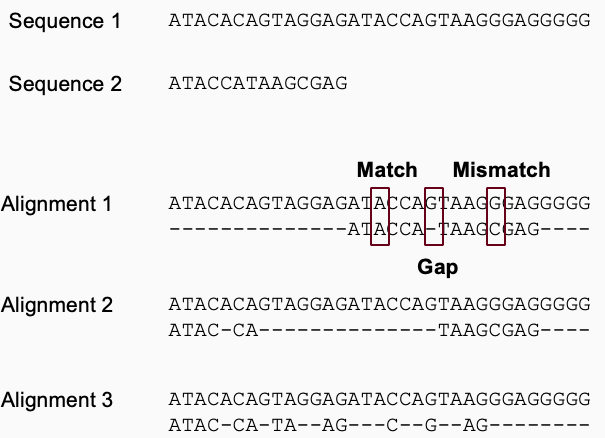
\includegraphics{figs/sequence_align.png}
\end{frame}

\begin{frame}{Scoring/Substitution Matrices}
\phantomsection\label{scoringsubstitution-matrices}
\Large

\begin{itemize}
\tightlist
\item
  Given alignment, how ``good'' is it?
\item
  Higher score = better alignment
\item
  Implicitly represent evolutionary patterns
\end{itemize}

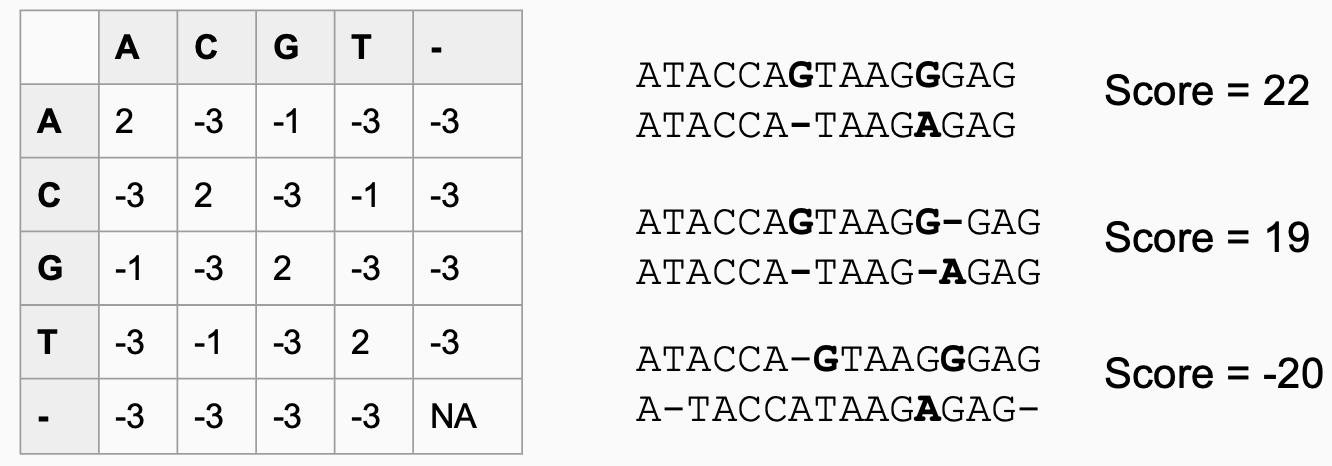
\includegraphics{figs/scoring.png}
\end{frame}

\begin{frame}{Sequence Alignment Algorithms}
\phantomsection\label{sequence-alignment-algorithms}
\Large

\begin{itemize}
\tightlist
\item
  \textbf{Global} alignments - beginning and end of both sequences must
  align
\item
  \textbf{Local} alignments - one sequence may align anywhere within the
  other
\item
  Multiplicity:

  \begin{itemize}
  \tightlist
  \item
    Pairwise alignments (2 sequences)
  \item
    Multiple sequence alignment (3+ sequences)
  \end{itemize}
\end{itemize}
\end{frame}

\begin{frame}{Global Alignment}
\phantomsection\label{global-alignment}
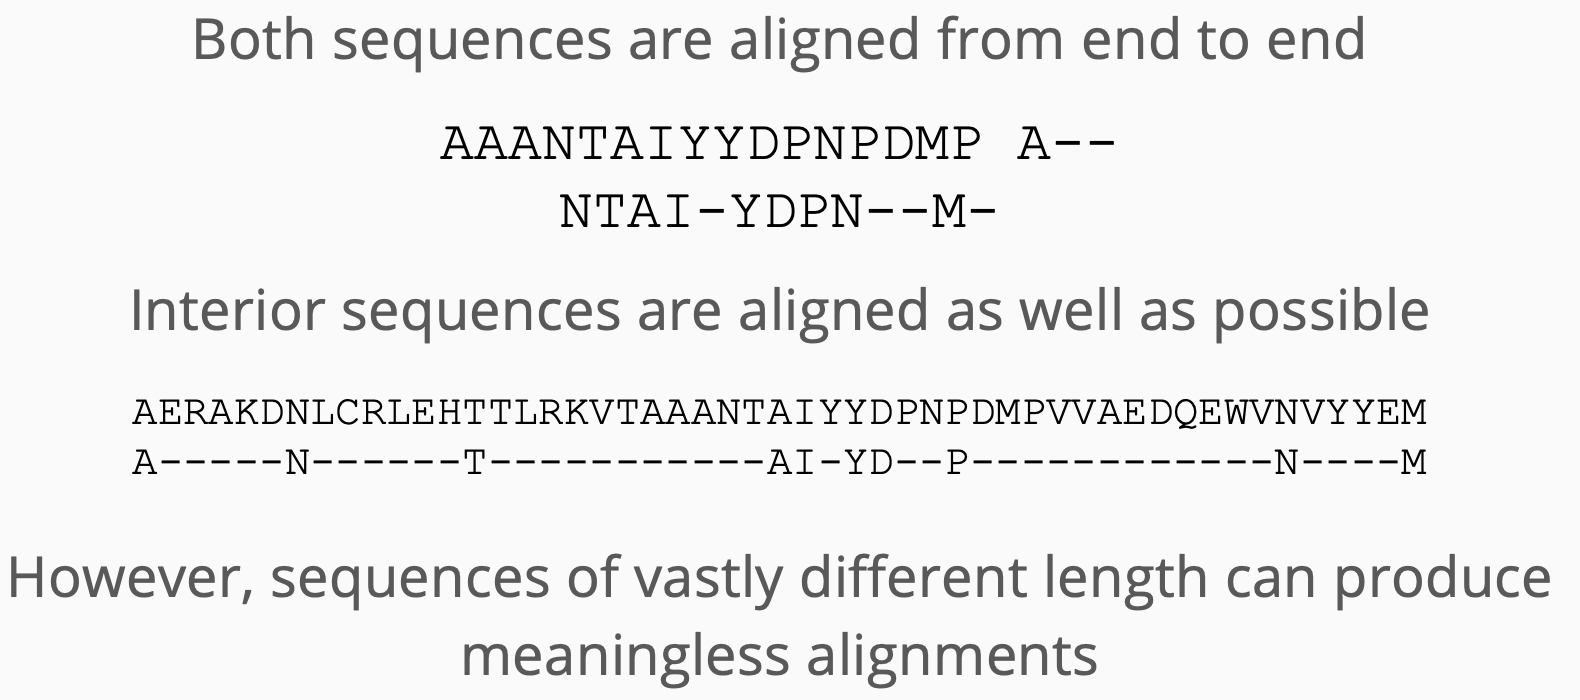
\includegraphics{figs/global_align.png}
\end{frame}

\begin{frame}{Local Alignment}
\phantomsection\label{local-alignment}
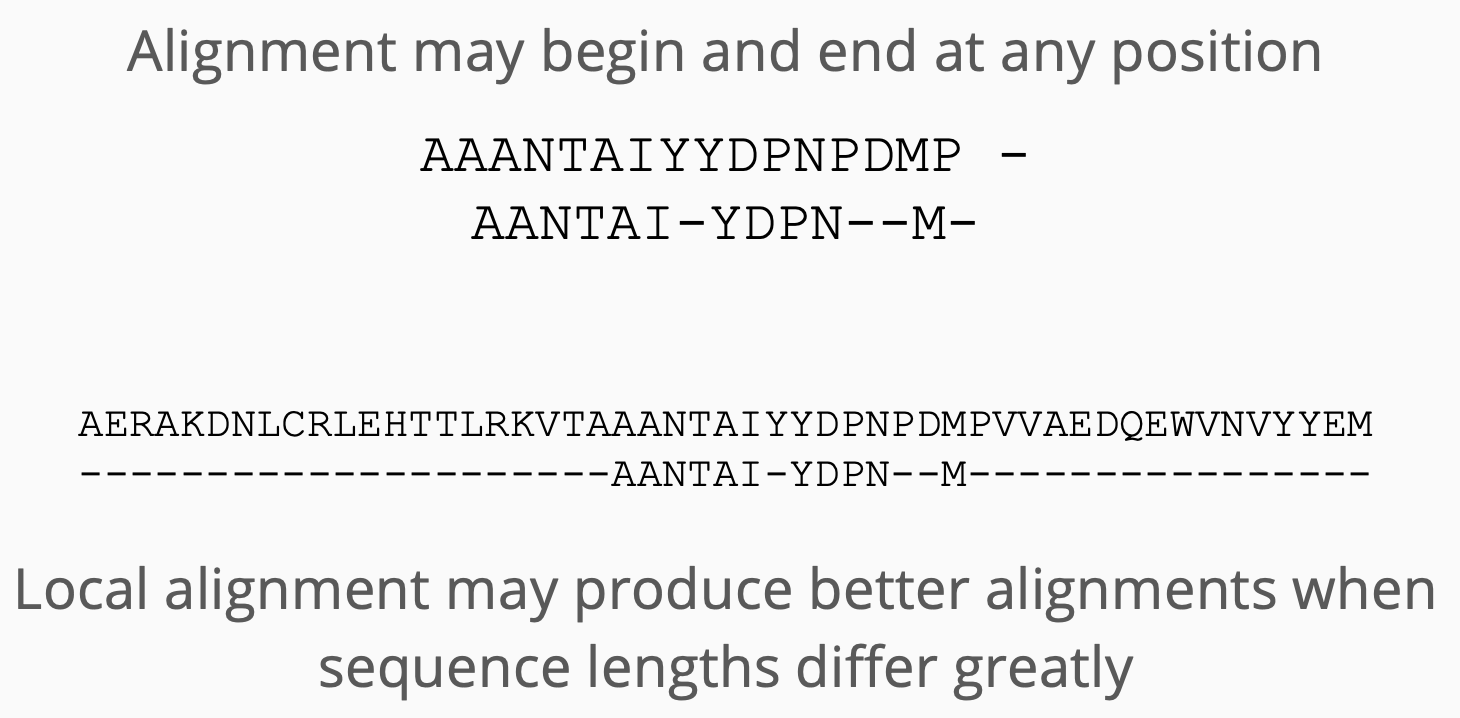
\includegraphics{figs/local_align.png}
\end{frame}

\begin{frame}{Multiple Sequence Alignment}
\phantomsection\label{multiple-sequence-alignment}
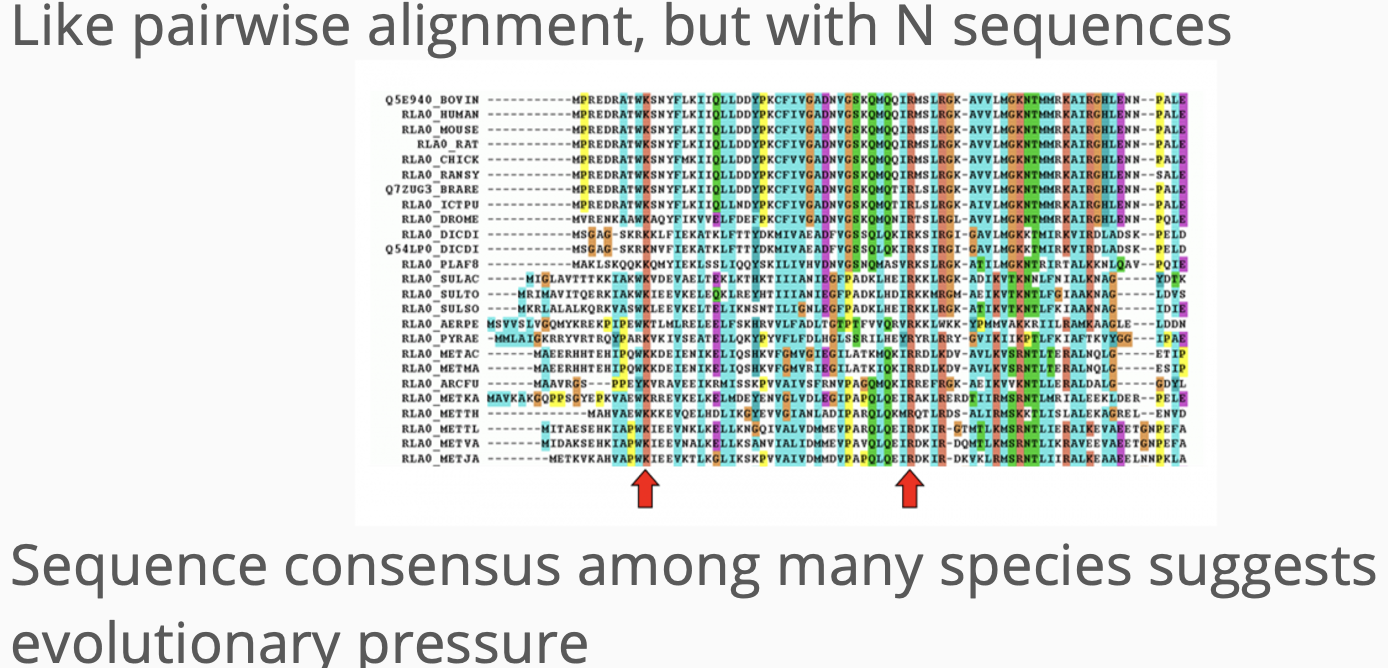
\includegraphics{figs/multiple_align.png}
\end{frame}

\begin{frame}{Methods for Multiple Sequence Aligment (MSA)}
\phantomsection\label{methods-for-multiple-sequence-aligment-msa}
\begin{enumerate}
\tightlist
\item
  \textbf{Progressive Alignment Algorithms}:

  \begin{itemize}
  \tightlist
  \item
    \emph{ClustalW}: A widely used progressive alignment tool with a
    guide tree strategy.
  \item
    \emph{Clustal Omega}: An enhanced version of ClustalW with improved
    speed and accuracy.
  \end{itemize}
\item
  \textbf{Iterative Alignment Algorithms}:

  \begin{itemize}
  \tightlist
  \item
    \emph{MAFFT (Multiple Alignment using Fast Fourier Transform)}: Uses
    iterative refinement with consistency scores.
  \item
    \emph{MUSCLE (Multiple Sequence Comparison by Log-Expectation)}:
    Utilizes progressive alignment followed by iterative refinement.
  \end{itemize}
\item
  \textbf{Hidden Markov Models (HMMs)}:

  \begin{itemize}
  \tightlist
  \item
    \emph{HMMER}: Based on HMMs, used for alignment and homology
    detection.
  \item
    \emph{SAM (Sequence Alignment and Modeling System)}: Combines HMMs
    with profiles for database searches.
  \end{itemize}
\end{enumerate}
\end{frame}

\begin{frame}{Methods for MSA (Continued)}
\phantomsection\label{methods-for-msa-continued}
\begin{enumerate}
\setcounter{enumi}{3}
\tightlist
\item
  \textbf{Probabilistic Alignment Methods}:

  \begin{itemize}
  \tightlist
  \item
    \emph{ProbCons}: Generates a probabilistic alignment using a
    Bayesian framework.
  \item
    \emph{PRANK}: Considers sequence and alignment uncertainty in
    alignment generation.
  \end{itemize}
\item
  \textbf{Structure-Based Alignment}:

  \begin{itemize}
  \tightlist
  \item
    \emph{MUSTANG (Multiple Structural Alignment by Secondary
    Structures)}: Aligns based on protein structures considering
    sequence and structure.
  \item
    \emph{DALI (Distance Alignment Matrix Method)}: Aligns sequences
    based on structural similarity.
  \end{itemize}
\end{enumerate}

These methods vary in their approaches and are chosen based on factors
such as alignment accuracy, computational efficiency, and the
characteristics of the input sequences.
\end{frame}

\begin{frame}{ClustalW: A Common MSA Tool}
\phantomsection\label{clustalw-a-common-msa-tool}
\Large

\begin{itemize}
\tightlist
\item
  ClustalW is one of the most widely used tools for multiple sequence
  alignment.
\item
  It uses a progressive alignment approach.
\item
  Available as standalone software or through
  \href{https://www.genome.jp/tools-bin/clustalw}{a web server}.
\end{itemize}
\end{frame}

\begin{frame}[fragile]{Example: Aligning TB genomes}
\phantomsection\label{example-aligning-tb-genomes}
\Large

Download the following TB genomes:

\begin{itemize}
\tightlist
\item
  \href{https://www.ncbi.nlm.nih.gov/nuccore/NC_000962.3?report=fasta}{H37Rv}
\item
  \href{https://www.ncbi.nlm.nih.gov/nuccore/AP012340.1?report=fasta}{Mycobacterium
  tuberculosis str. Erdman}
\item
  Combine into single FASTA, first 100 lines:
\end{itemize}

\normalsize

\begin{Shaded}
\begin{Highlighting}[]
\KeywordTok{\{} \FunctionTok{head} \AttributeTok{{-}101}\NormalTok{ sequence.fasta}\KeywordTok{;} \FunctionTok{head} \AttributeTok{{-}101}\NormalTok{ sequence{-}2.fasta}\KeywordTok{;} \KeywordTok{\}} \DataTypeTok{\textbackslash{}}
\OperatorTok{\textgreater{}}\NormalTok{ combined.fasta}
\end{Highlighting}
\end{Shaded}

\Large

\begin{itemize}
\tightlist
\item
  Analyze using
  \href{https://www.genome.jp/tools-bin/clustalw}{ClustalW}
\end{itemize}
\end{frame}

\begin{frame}{Example: Genome Assembly}
\phantomsection\label{example-genome-assembly}
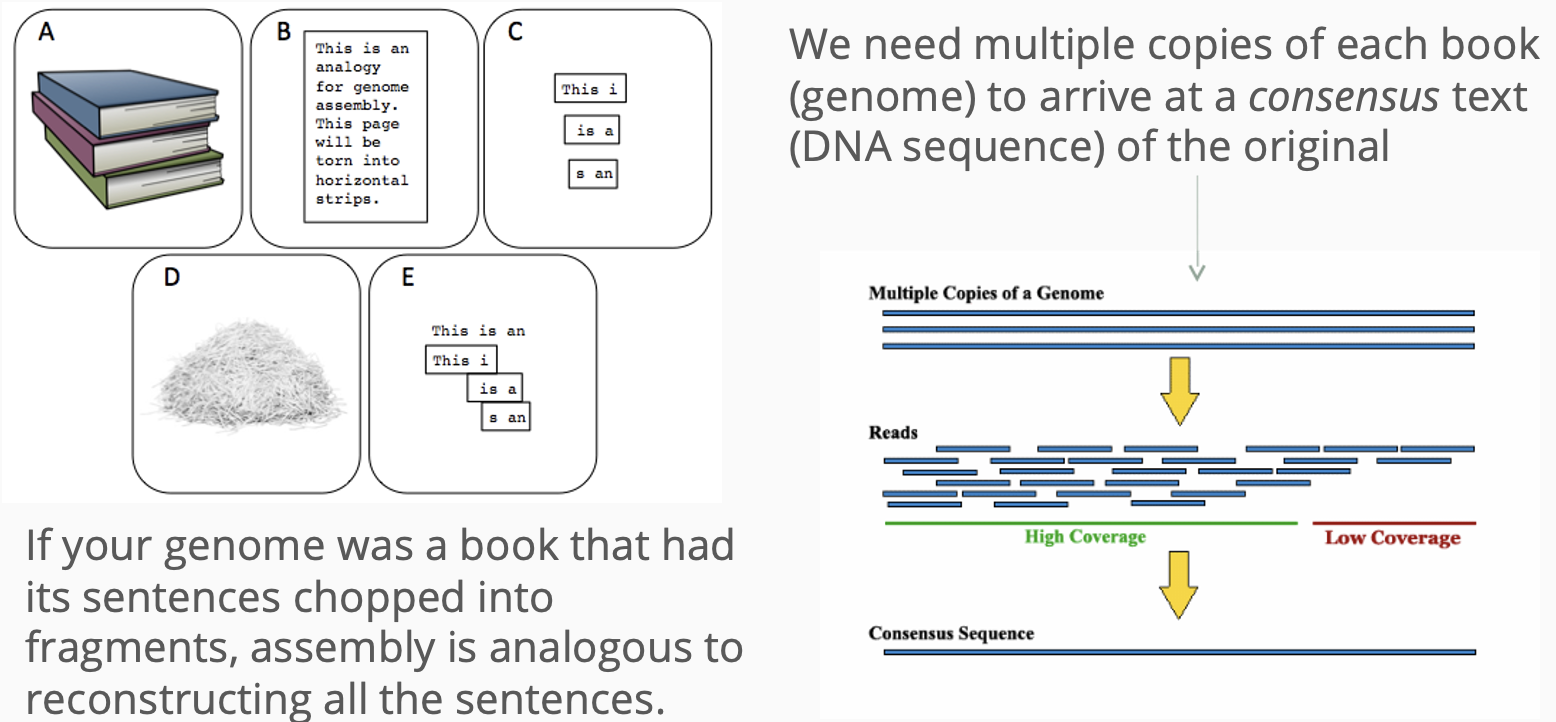
\includegraphics{figs/assembly.png}
\end{frame}

\begin{frame}{Example: Genome Assembly}
\phantomsection\label{example-genome-assembly-1}
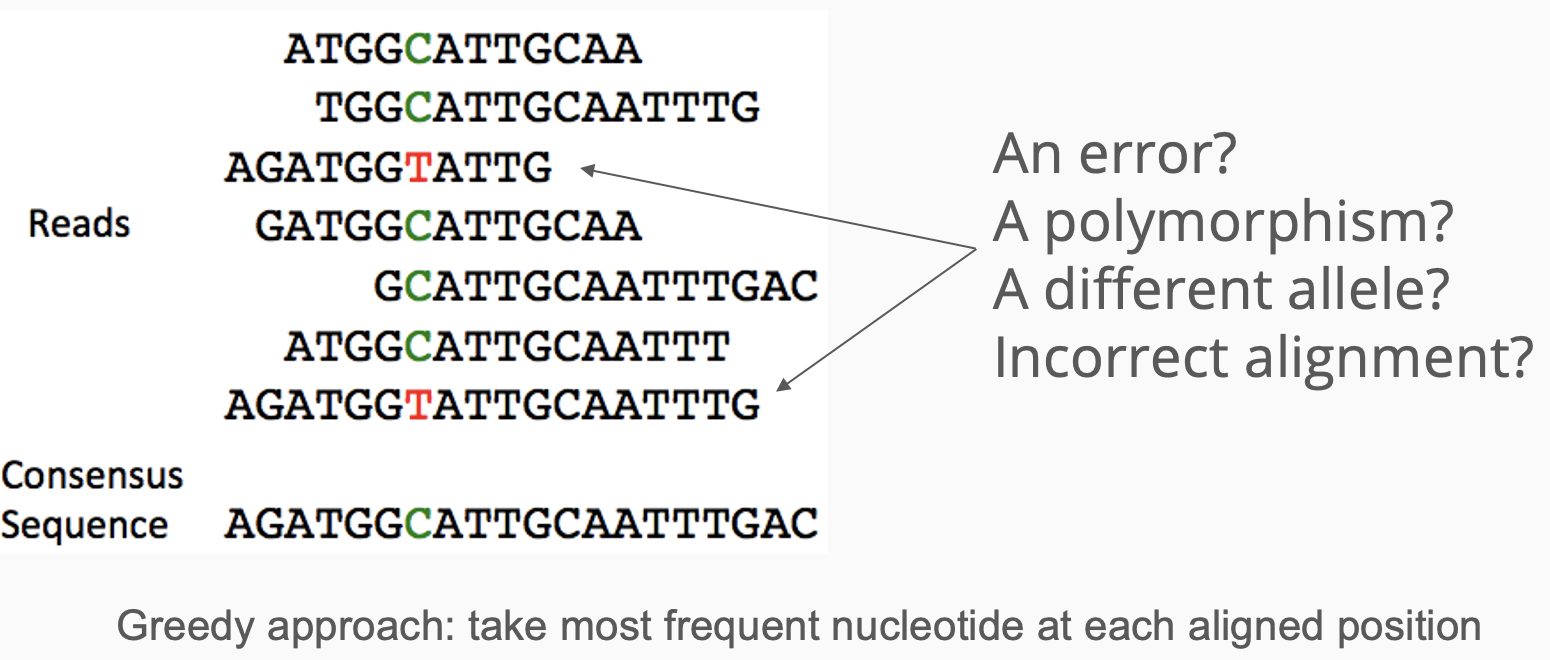
\includegraphics{figs/assembly2.png}
\end{frame}

\begin{frame}{Example: mRNA-Seq Analysis}
\phantomsection\label{example-mrna-seq-analysis}
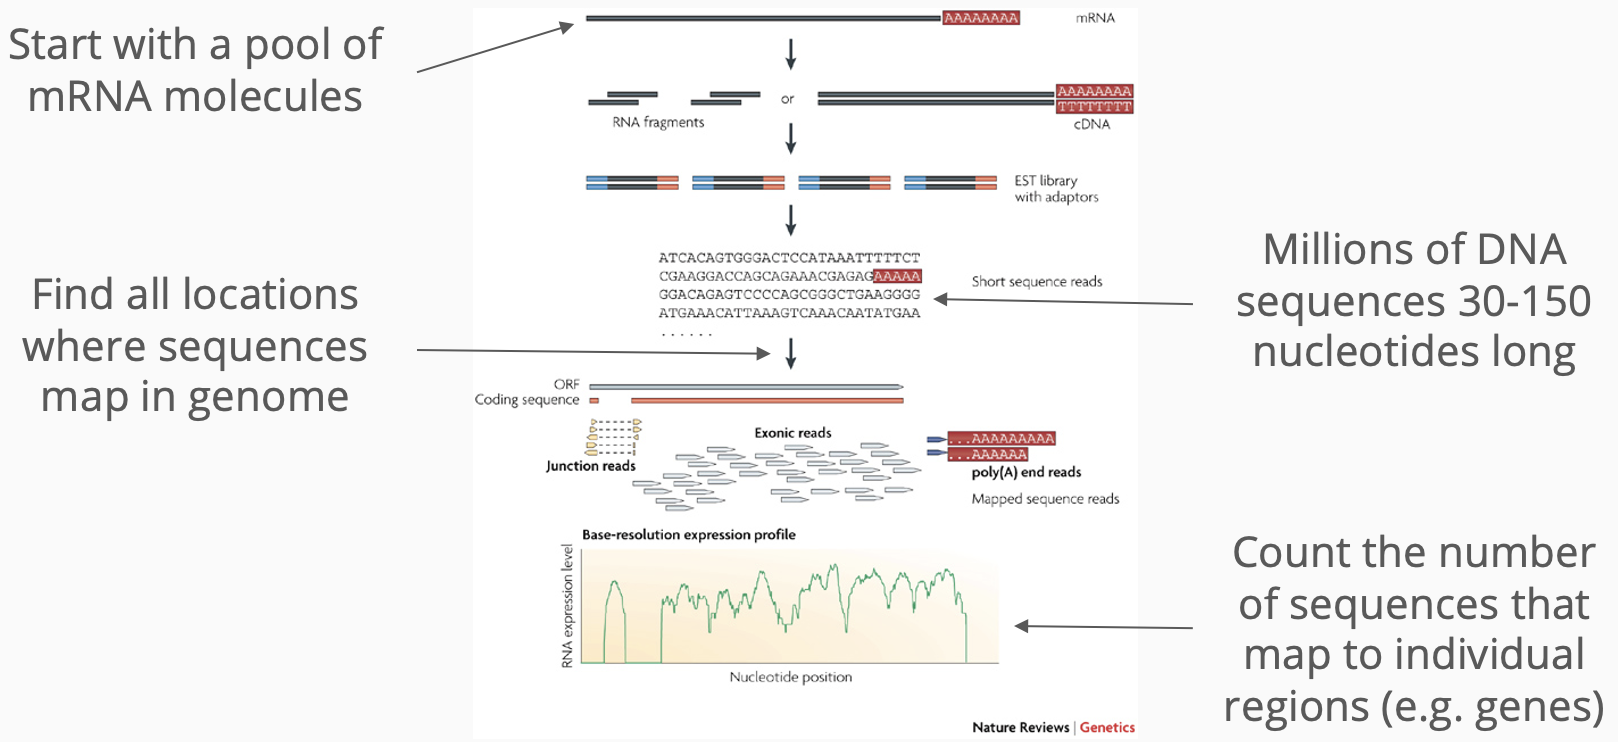
\includegraphics{figs/rnaseq_assemble.png}
\end{frame}

\begin{frame}{Example: DNA Binding Site Discovery}
\phantomsection\label{example-dna-binding-site-discovery}
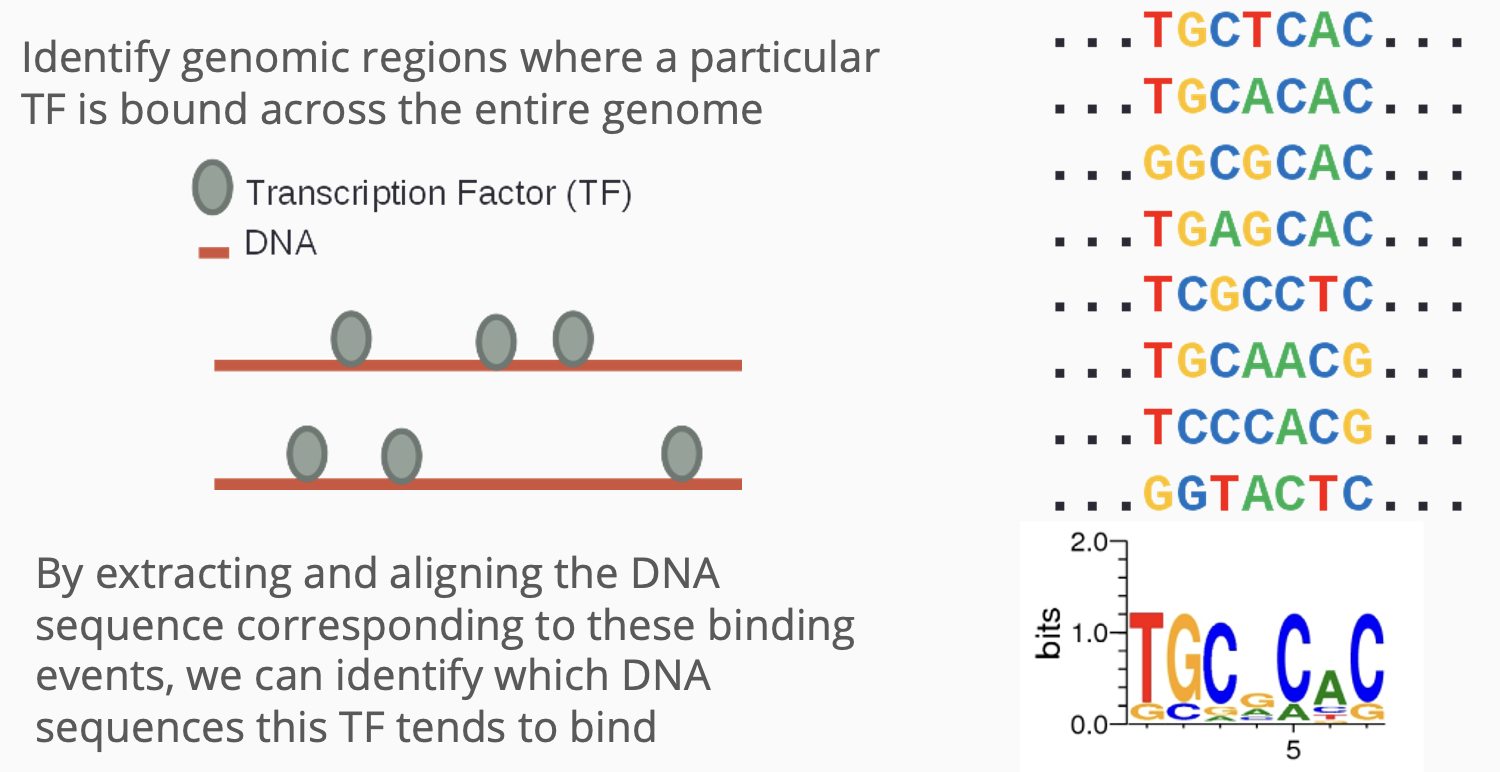
\includegraphics{figs/binding_assemble.png}
\end{frame}

\section{Whole Genome/Exome
Sequencing}\label{whole-genomeexome-sequencing}

\begin{frame}{Whole Genome Sequencing}
\phantomsection\label{whole-genome-sequencing}
\Large

\begin{itemize}
\tightlist
\item
  \textbf{W}hole \textbf{G}enome \textbf{S}equencing (WGS)
\item
  Generate enough reads to attain:

  \begin{itemize}
  \tightlist
  \item
    More than 95\% coverage of source genome
  \item
    More than 30x average depth
  \end{itemize}
\item
  Two strategies:

  \begin{itemize}
  \tightlist
  \item
    De novo: assemble reads into a new sequence
  \item
    Re-sequence: refine an existing reference sequence
  \end{itemize}
\end{itemize}
\end{frame}

\begin{frame}{De novo assembly}
\phantomsection\label{de-novo-assembly}
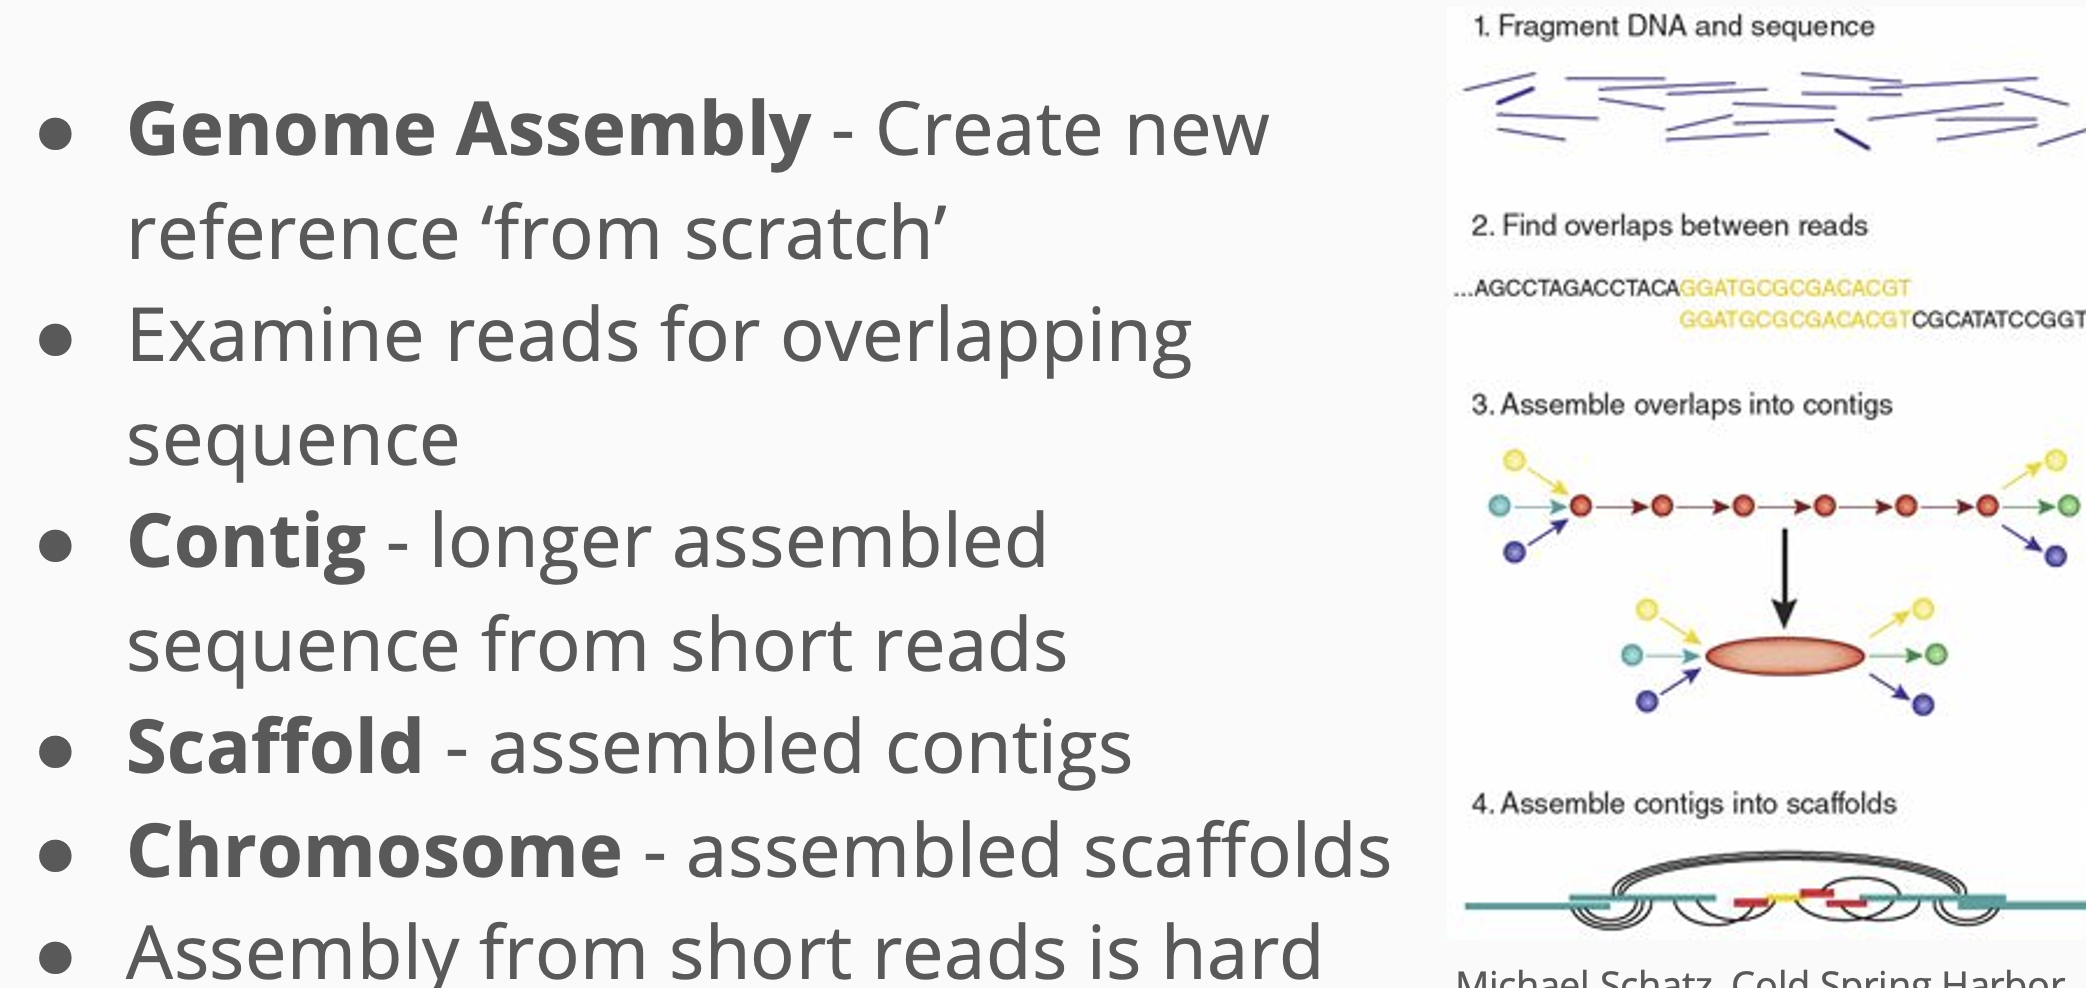
\includegraphics{figs/denovo.png}
\end{frame}

\begin{frame}{De novo assembly: graph-based}
\phantomsection\label{de-novo-assembly-graph-based}
\Large

\begin{itemize}
\tightlist
\item
  Greedy assembly creates linear sequences
\item
  Vulnerable to finding local optima
\item
  Graph representation considers all sequence content simultaneously
\item
  Graph data structure can encode variability (e.g.~insertions, SNPs)
\item
  Computationally much more expensive
\item
  de Brujin Graphs and Overlap Layout Consensus
\end{itemize}
\end{frame}

\begin{frame}{De novo assembly: graph-based}
\phantomsection\label{de-novo-assembly-graph-based-1}
\center

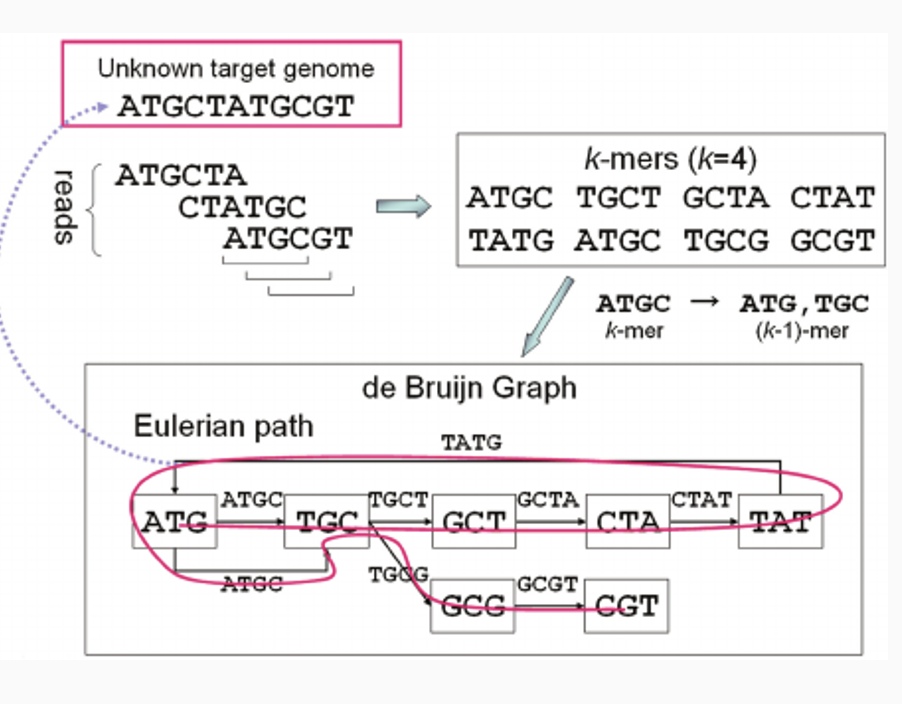
\includegraphics[width=\textwidth,height=0.8\textheight]{figs/denovograph.png}
\end{frame}

\begin{frame}{Reference guided genome assembly}
\phantomsection\label{reference-guided-genome-assembly}
\Large

\begin{itemize}
\tightlist
\item
  Refine existing reference with new sequence
\item
  Can discover:

  \begin{itemize}
  \tightlist
  \item
    New structural variants
  \item
    Novel insertions/alternate haplotypes or scaffolds
  \item
    Polymorphisms
  \end{itemize}
\item
  Faster, easier than de novo assembly
\item
  More sensitive to existing biases in reference
\end{itemize}
\end{frame}

\begin{frame}{Reference guided genome assembly}
\phantomsection\label{reference-guided-genome-assembly-1}
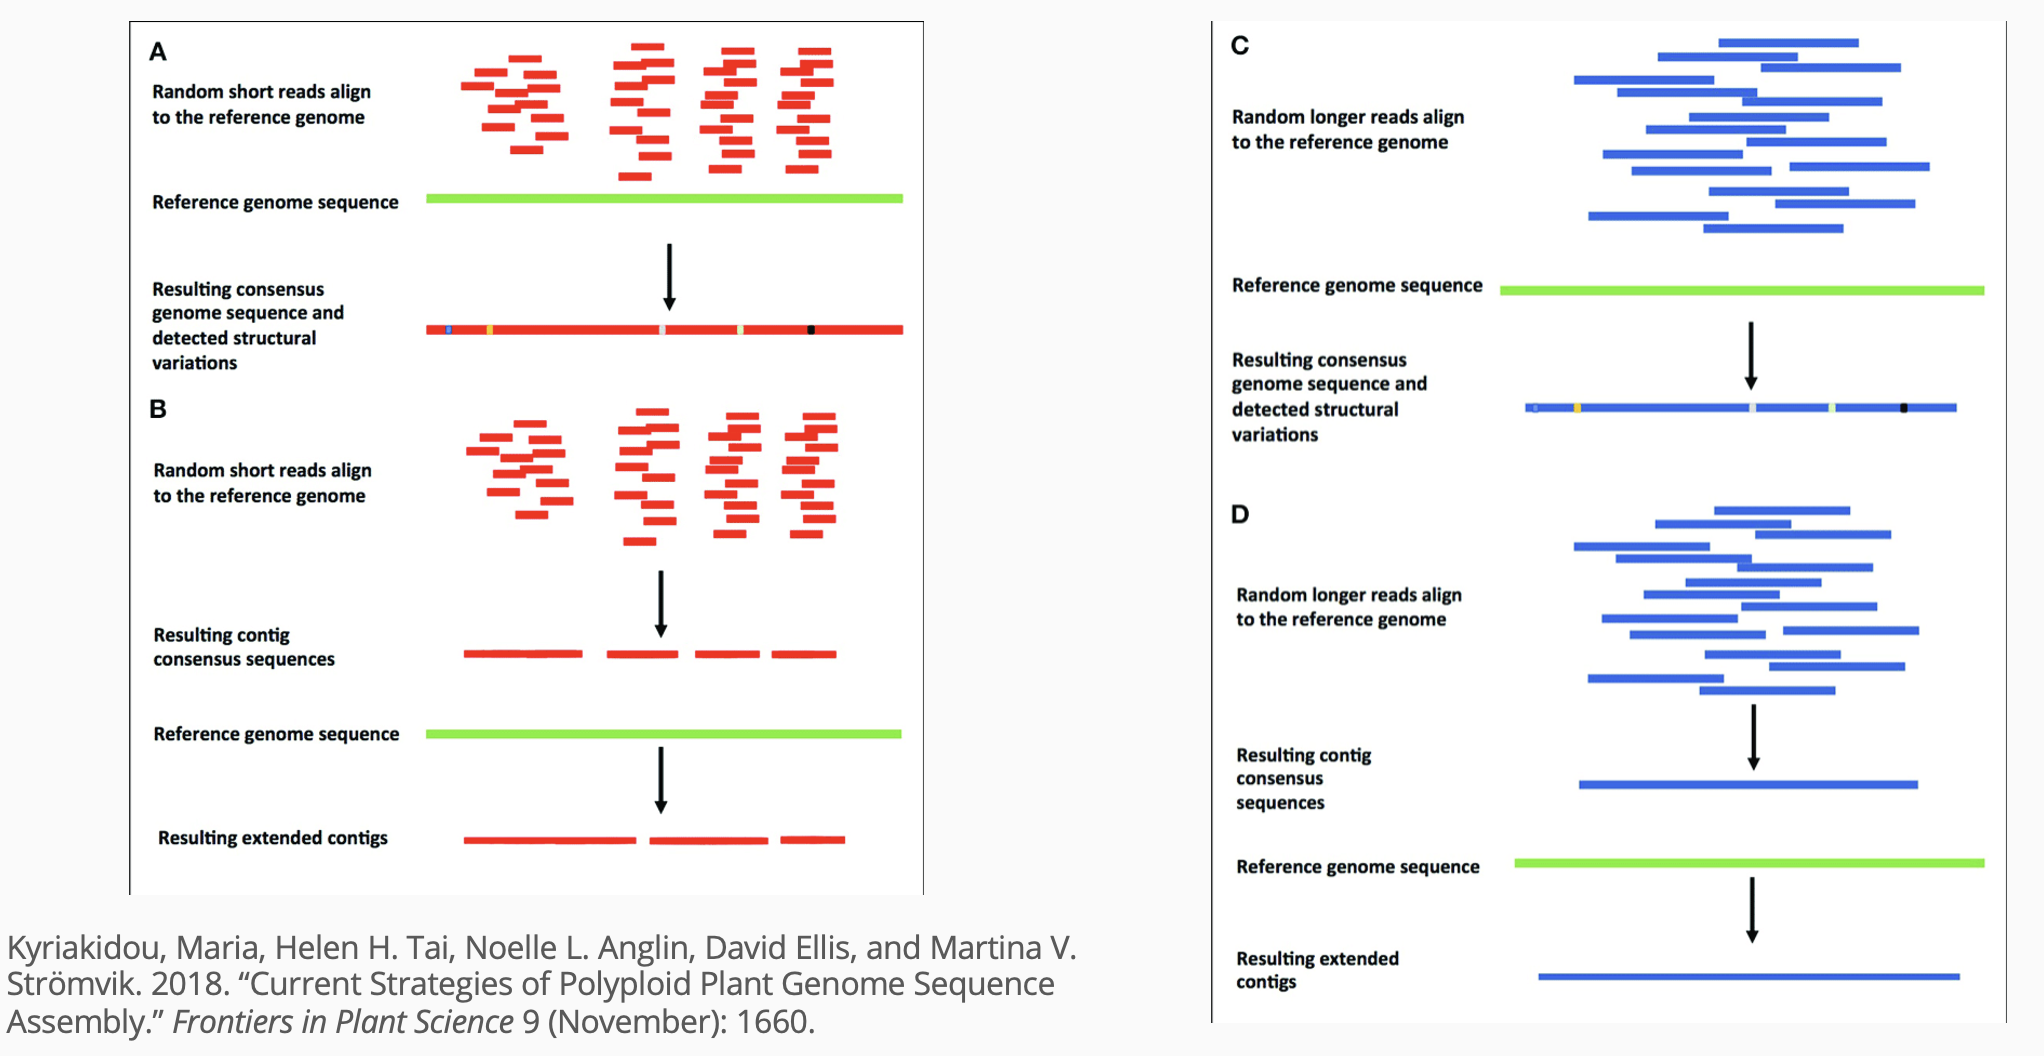
\includegraphics{figs/reference_assemble.png}
\end{frame}

\begin{frame}{Whole Exome Sequencing}
\phantomsection\label{whole-exome-sequencing}
\Large

\begin{itemize}
\tightlist
\item
  \textbf{W}hole \textbf{E}xome \textbf{S}equencing (WES)
\item
  Exons 1\%-2\% of human genome sequence
\item
  Pre-select reads that map to exons
\item
  Sequence to much greater depth than WGS
\item
  Identify coding variants
\end{itemize}
\end{frame}

\begin{frame}{Exome Sequence Selection}
\phantomsection\label{exome-sequence-selection}
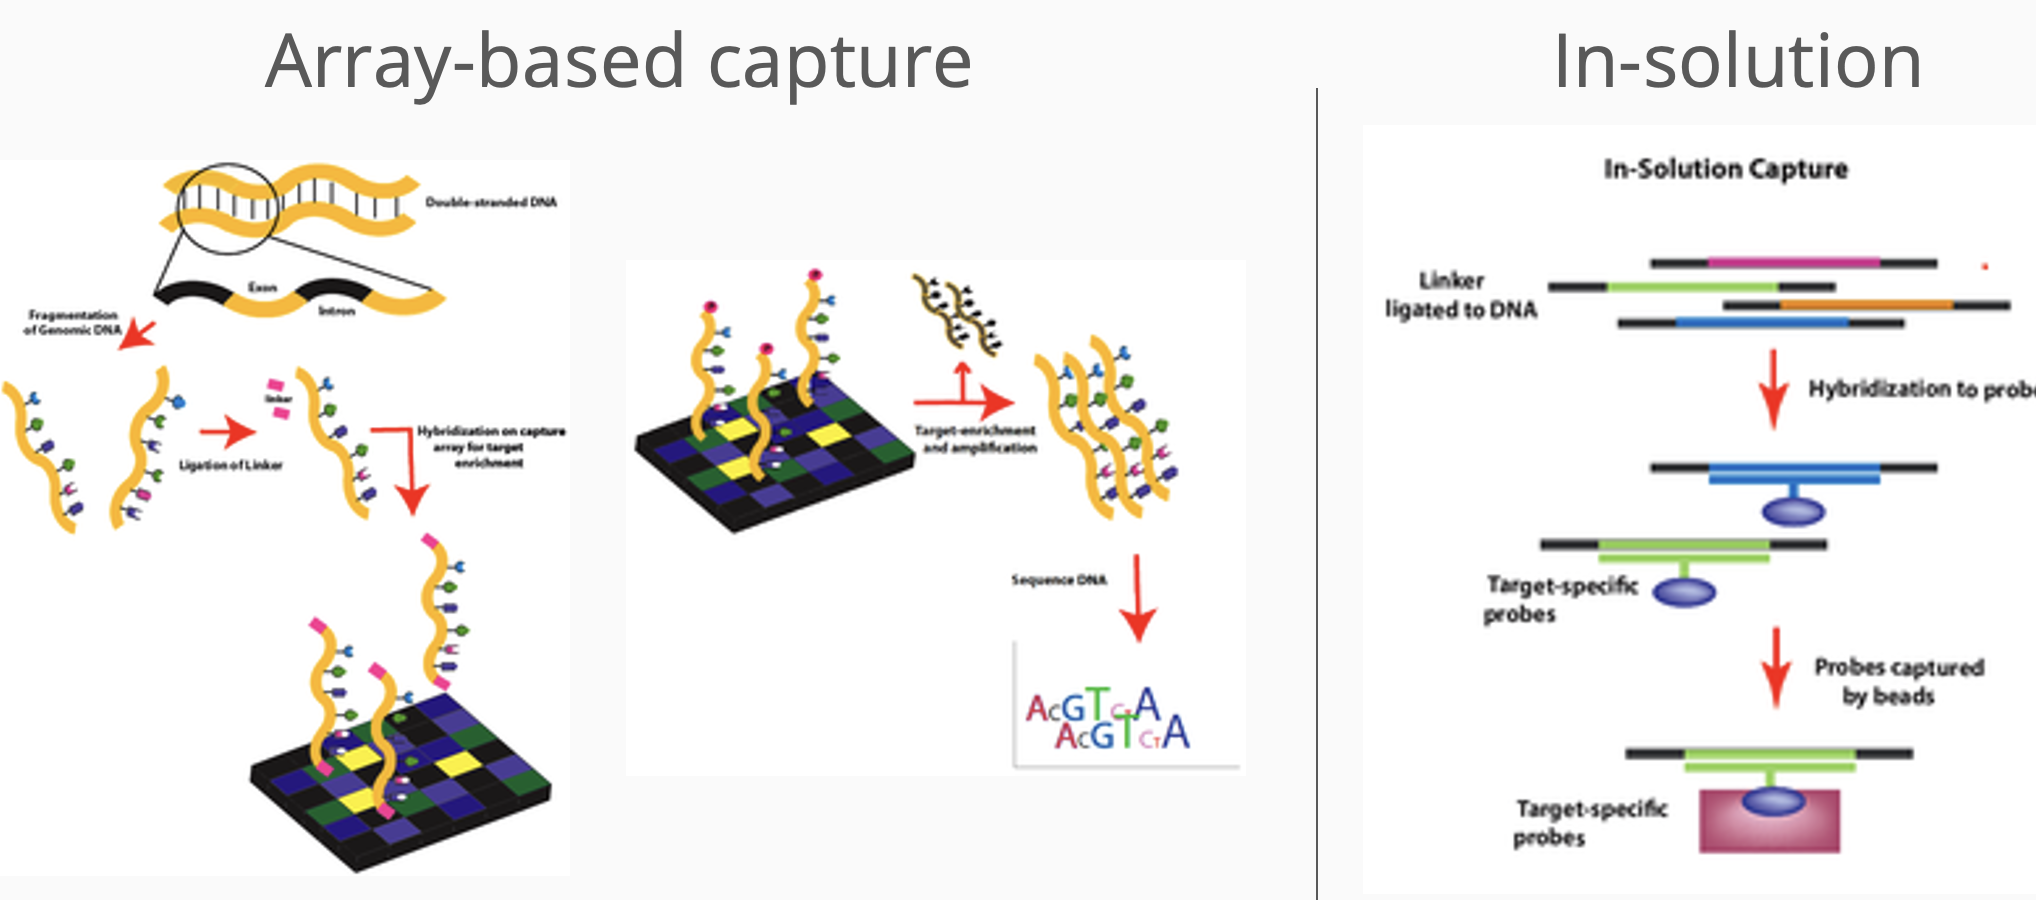
\includegraphics{figs/exome_selection.png}
\end{frame}

\section{SNP and Variant Calling}\label{snp-and-variant-calling}

\begin{frame}{Genomic Variants}
\phantomsection\label{genomic-variants}
\Large

\begin{itemize}
\tightlist
\item
  Individual genomes from same species vary
\item
  WGS/WES compared with reference can identify differences
\item
  \textbf{Variant}: sequence that varies within species
\item
  Two general types:

  \begin{itemize}
  \tightlist
  \item
    Small: \textless50 bp, single nucleotide polymorphisms (SNPs),
    indels
  \item
    Large: \textgreater50 bp, copy number variations, duplications,
    deletions, translocations, inversions
  \end{itemize}
\end{itemize}
\end{frame}

\begin{frame}{Genomic Variants}
\phantomsection\label{genomic-variants-1}
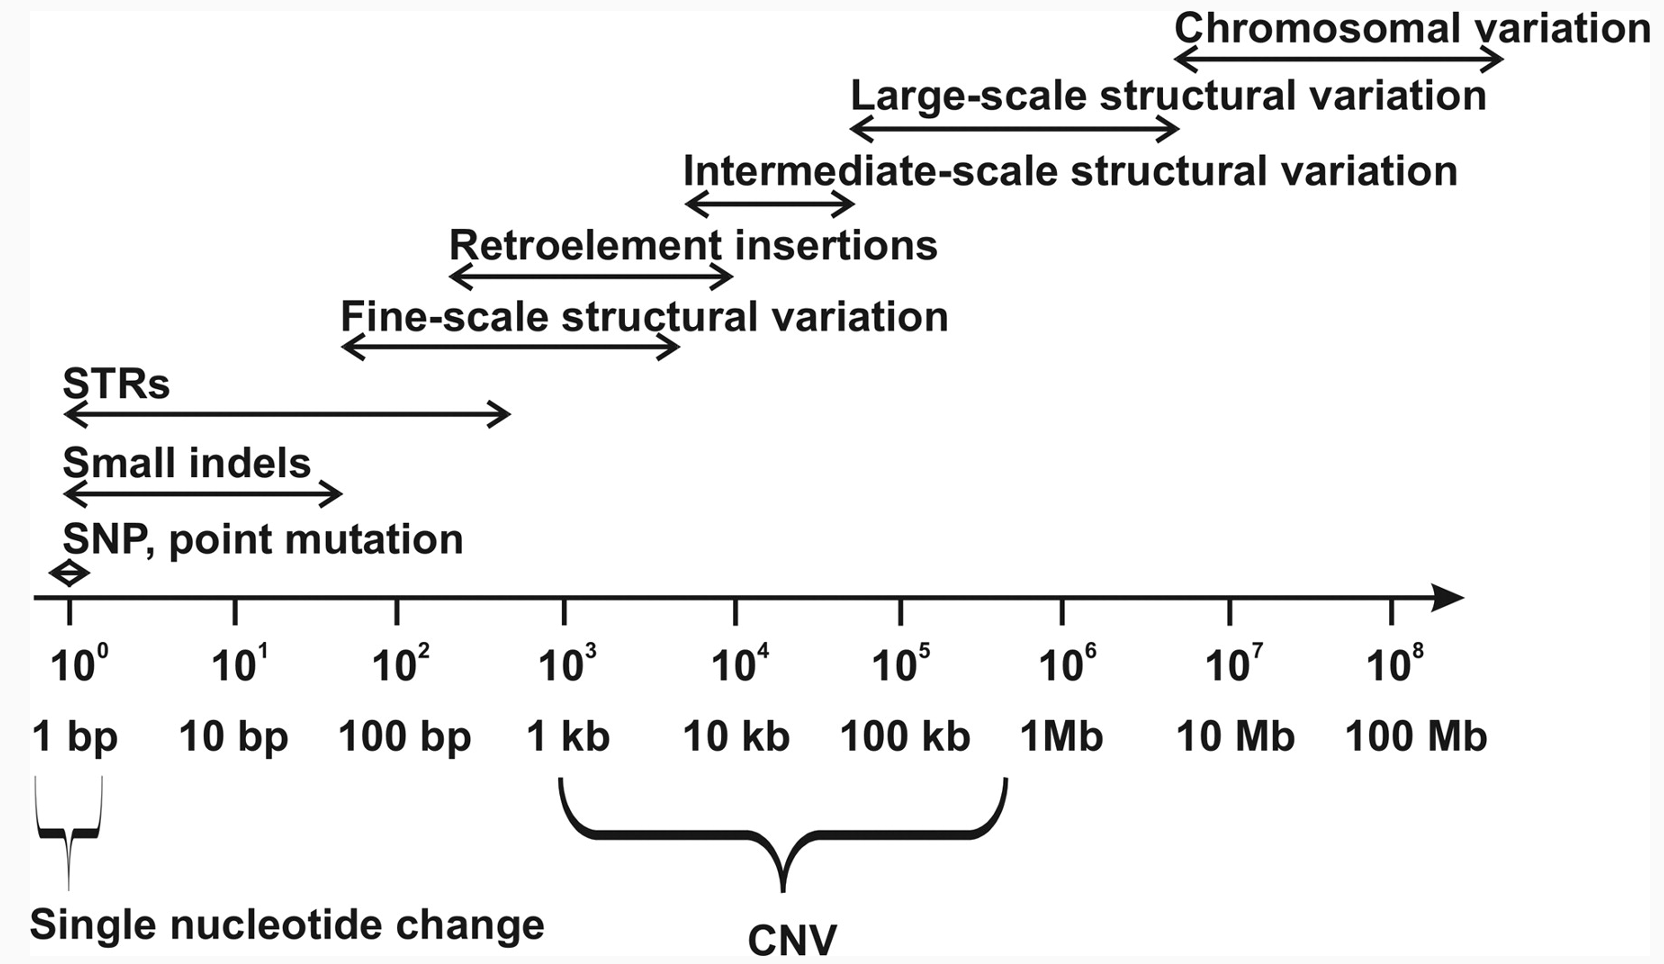
\includegraphics{figs/variant_defs.png}
\end{frame}

\begin{frame}{Point mutations}
\phantomsection\label{point-mutations}
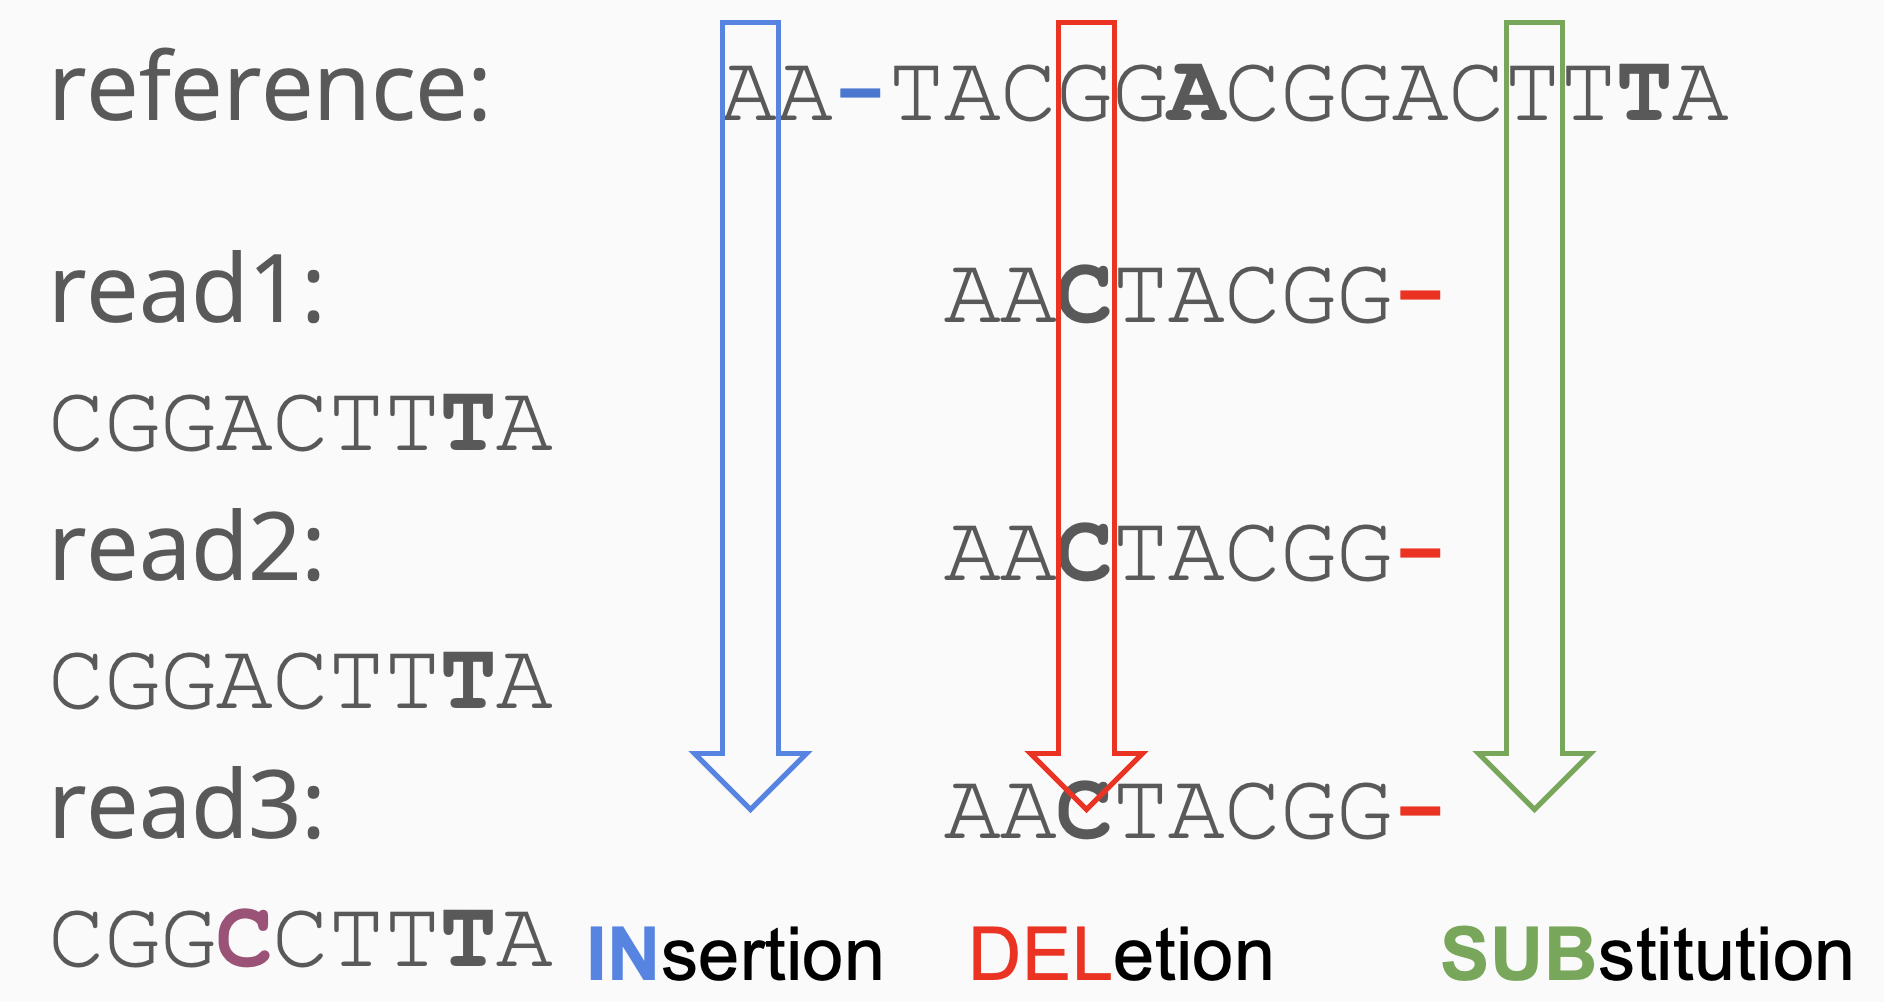
\includegraphics{figs/point_mut.png}
\end{frame}

\begin{frame}{Single Nucleotide Polymorphisms (SNPs)}
\phantomsection\label{single-nucleotide-polymorphisms-snps}
\Large

\begin{itemize}
\tightlist
\item
  Most commonly studied type of variant
\item
  Types of single nucleotide alterations:

  \begin{itemize}
  \tightlist
  \item
    \textbf{Variant} (SNV) - any single mutation
  \item
    \textbf{Polymorphism} (SNP) - SNV observed in significant frequency
    in population (e.g.~\textgreater1\%)
  \end{itemize}
\item
  Typically base changes, e.g.~A to C
\item
  SNPs (usually) indicate shared ancestry
\item
  May suggest disease mechanism
\end{itemize}
\end{frame}

\begin{frame}{Structural variation}
\phantomsection\label{structural-variation}
\Large

\begin{itemize}
\tightlist
\item
  Deletions - sequence missing
\item
  Insertions:

  \begin{itemize}
  \tightlist
  \item
    Novel - new sequence added
  \item
    Mobile-element - copied/moved from elsewhere in genome
  \end{itemize}
\item
  Duplications:

  \begin{itemize}
  \tightlist
  \item
    Tandem - consecutive
  \item
    Interspersed - non-consecutive
  \end{itemize}
\item
  Inversion - segment is reversed
\item
  Translocation - segment moves
\end{itemize}
\end{frame}

\begin{frame}{Structural variation}
\phantomsection\label{structural-variation-1}
\center

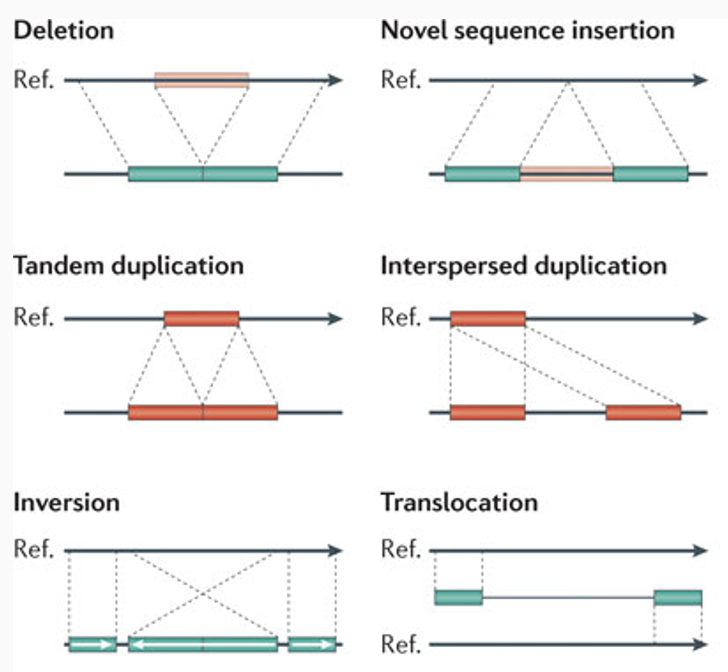
\includegraphics[width=\textwidth,height=0.8\textheight]{figs/struc_vars.png}
\end{frame}

\begin{frame}{Genotyping}
\phantomsection\label{genotyping}
\Large

\begin{itemize}
\tightlist
\item
  \textbf{Genotype}: an individual's variant(s)
\item
  \textbf{Phenotype}: an individual's physical form
\item
  \textbf{De novo} variant calling/detection: given genomic reads and a
  reference, find all the variants
\item
  \textbf{Genotyping}: examine individual for \emph{a priori} variants
  at known locations

  \begin{itemize}
  \tightlist
  \item
    Can use arrays (i.e.~SNP Chip) or WGS/WES
  \end{itemize}
\end{itemize}
\end{frame}

\begin{frame}{Human Genomic Variants}
\phantomsection\label{human-genomic-variants}
\Large

\begin{itemize}
\tightlist
\item
  Humans have diploid genome

  \begin{itemize}
  \tightlist
  \item
    i.e.~2 copies of each gene
  \end{itemize}
\item
  dbSNP - NCBI repository for SNPs

  \begin{itemize}
  \tightlist
  \item
    As of June 2021 (Build 155)
  \item
    3.3B submitted variants
  \item
    1B annotated human SNPs Every human has on average:
  \item
    A variant every 1kb
  \item
    2-3 million SNPs
  \end{itemize}
\end{itemize}
\end{frame}

\begin{frame}{Human Genomic Terminology}
\phantomsection\label{human-genomic-terminology}
\Large

\begin{itemize}
\tightlist
\item
  \textbf{Allele}: sequence containing a variant
\item
  \textbf{Homozygous variant}: both same allele

  \begin{itemize}
  \tightlist
  \item
    i.e.~either same variant or same as reference
  \end{itemize}
\item
  \textbf{Heterozygous variant}: different alleles

  \begin{itemize}
  \tightlist
  \item
    i.e.~one is variant, one is reference/different variant
  \end{itemize}
\end{itemize}

\center

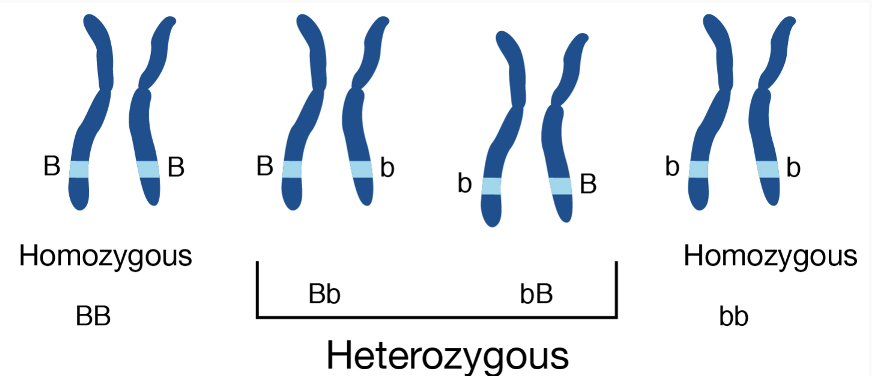
\includegraphics[width=0.7\textwidth,height=\textheight]{figs/human_genomic.png}
\url{https://www.genome.gov/genetics-glossary/heterozygous}
\end{frame}

\begin{frame}{Human Genomic Terminology}
\phantomsection\label{human-genomic-terminology-1}
\Large

For coding (exonic) variants:

\begin{itemize}
\tightlist
\item
  \textbf{Synonymous or sense}: variant does not change amino acid
  sequence
\item
  \textbf{Non-synonymous or mis-sense}: variant causes amino acid change
\item
  \textbf{Non-sense}: causes early termination of protein by introducing
  stop codon
\item
  \textbf{Frameshift}: insertion or deletion causes complete recoding of
  downstream proteins
\end{itemize}
\end{frame}

\begin{frame}{Genomic Variant Terminology}
\phantomsection\label{genomic-variant-terminology}
\Large

\begin{itemize}
\tightlist
\item
  \textbf{Germline}: Inherited from parents

  \begin{itemize}
  \tightlist
  \item
    e.g.~blue eyes, familial disease risk
  \end{itemize}
\item
  \textbf{Somatic}: Acquired during life

  \begin{itemize}
  \tightlist
  \item
    e.g.~tumor vs normal tissue
  \end{itemize}
\item
  \textbf{Allele frequency}: how common is a given variant in some
  population, e.g.:

  \begin{itemize}
  \tightlist
  \item
    1\% of human population
  \item
    30\% within people with some disease
  \end{itemize}
\end{itemize}
\end{frame}

\begin{frame}{dbSNP - NCBI SNP Database}
\phantomsection\label{dbsnp---ncbi-snp-database}
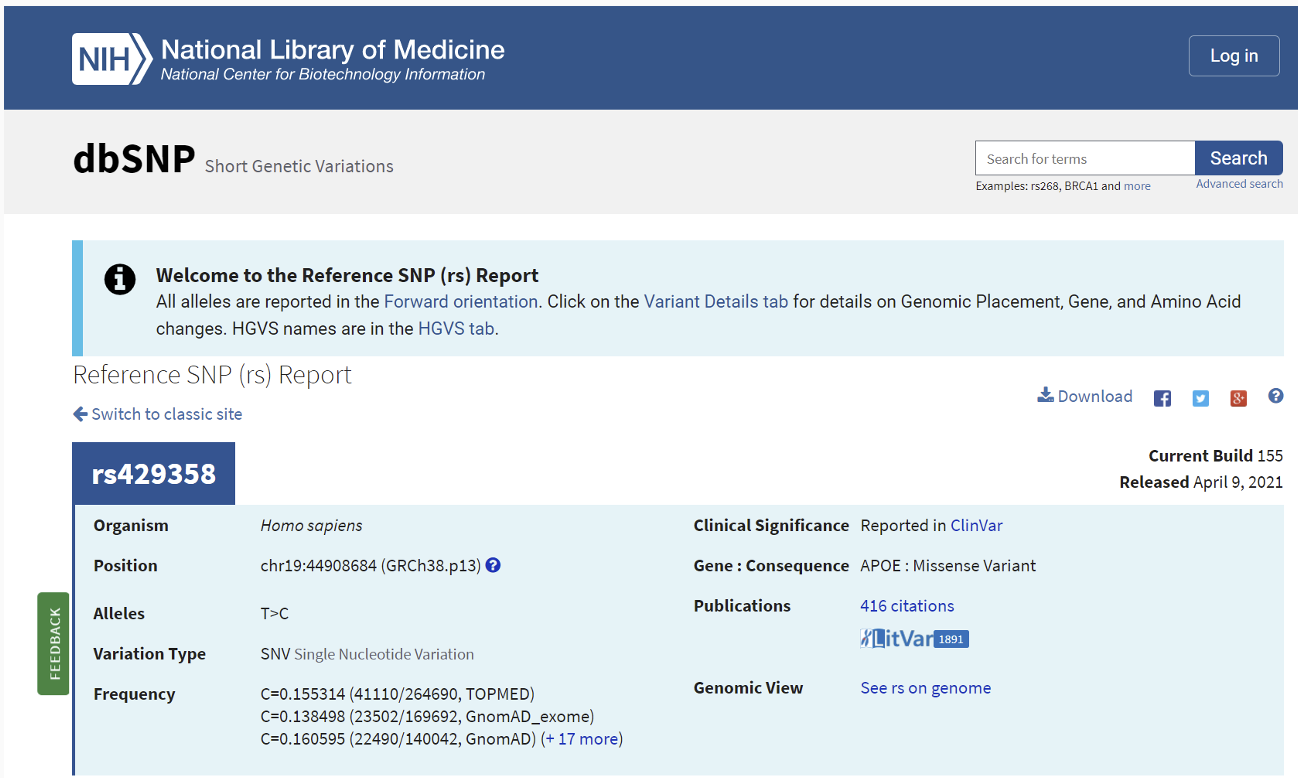
\includegraphics{figs/dbsnp.png} \#\# Variants Smaller Than A Read

\Large

\begin{itemize}
\tightlist
\item
  Finding SNPs, indels almost a solved problem
\item
  SNPs called are 95\% accurate

  \begin{itemize}
  \tightlist
  \item
    i.e.~with sufficient coverage
  \end{itemize}
\item
  Structural variants cause false positives
\item
  Duplications, somatic mutations may cause 3 or more alleles to be
  observed
\end{itemize}
\end{frame}

\begin{frame}{SNP and indel density is non-random}
\phantomsection\label{snp-and-indel-density-is-non-random}
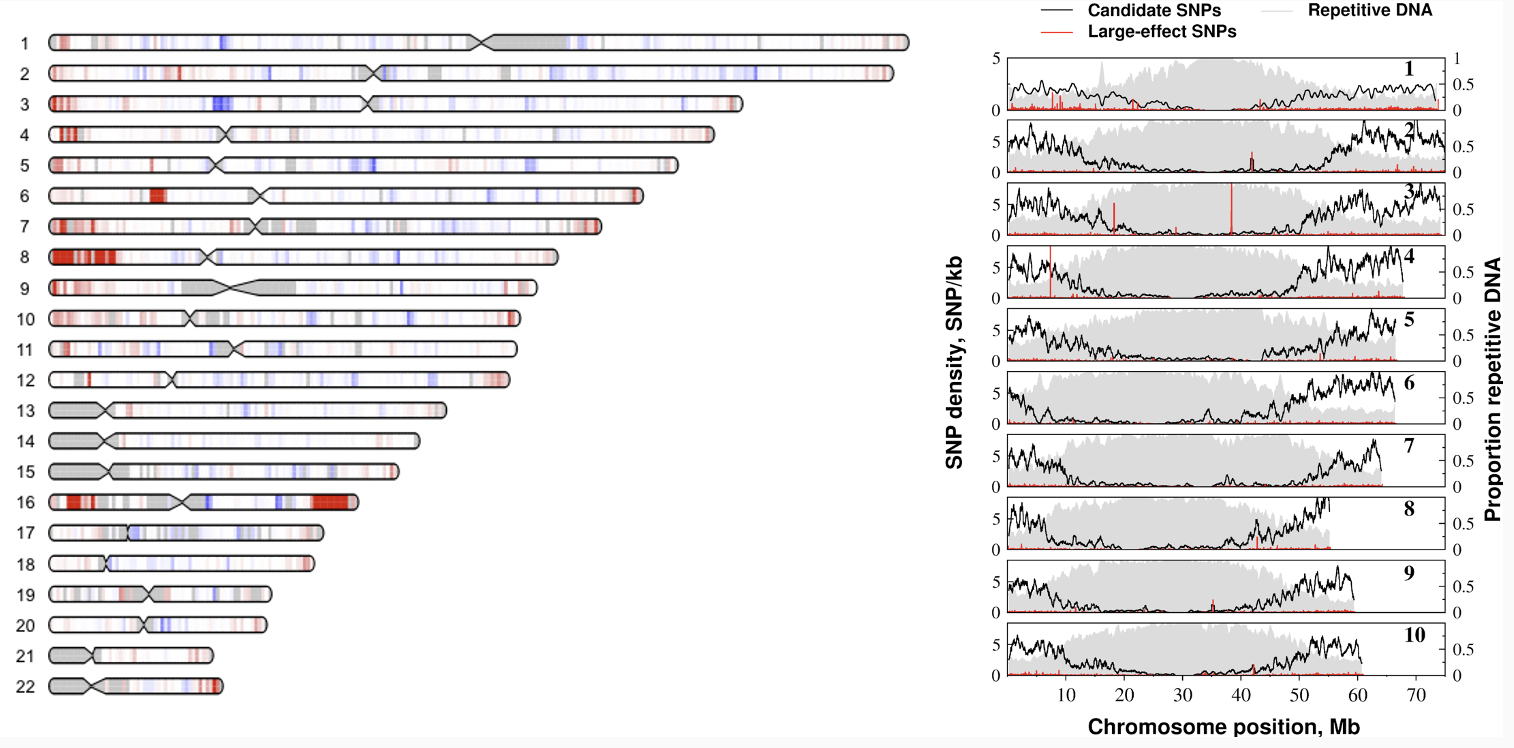
\includegraphics{figs/snp_density.png}
\end{frame}

\begin{frame}{Variants Larger Than A Read}
\phantomsection\label{variants-larger-than-a-read}
\Large

\begin{itemize}
\tightlist
\item
  \textbf{Structural Variation (SV)}
\item
  Two types:

  \begin{itemize}
  \tightlist
  \item
    Balanced - Do not change amount of DNA
  \item
    Copy Number Variants (CNV) - Change amount of DNA Scales:
  \item
    Mini (hundreds of basepairs)
  \item
    Macro (visible by a microscope) variants
  \item
    Much harder to find (especially balanced) Non-random: SV `hotspots'
  \end{itemize}
\end{itemize}
\end{frame}

\begin{frame}{Haplotyping}
\phantomsection\label{haplotyping}
\Large

\begin{itemize}
\tightlist
\item
  DNA recombines in large blocks
\item
  SNPs in a block move around together
\item
  Looking at the common SNPs in a block, reveals the ancestry
  information
\item
  \textbf{Linkage Disequilibrium (LD)}: adjacent SNPs co-occur more
  often than expected

  \begin{itemize}
  \tightlist
  \item
    i.e.~2 SNPs are in LD with each other
  \end{itemize}
\end{itemize}
\end{frame}

\begin{frame}{Haplotyping}
\phantomsection\label{haplotyping-1}
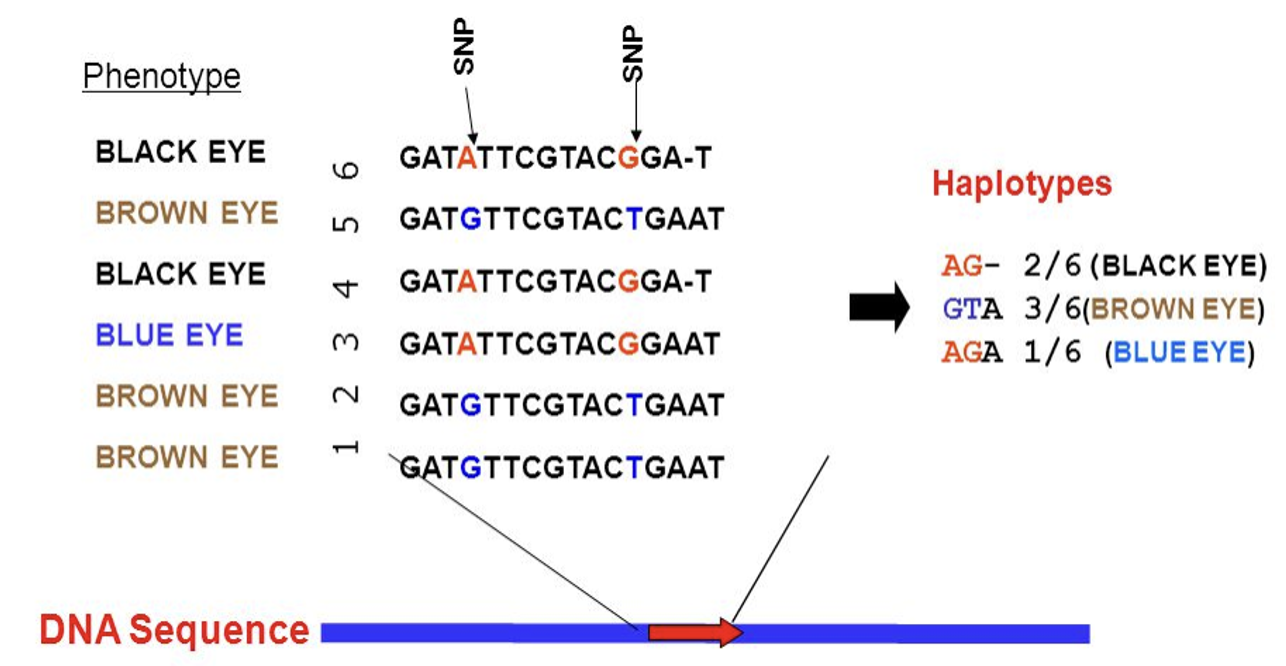
\includegraphics{figs/haplotype.png}
\end{frame}

\begin{frame}{Methods for SNP Calling}
\phantomsection\label{methods-for-snp-calling}
\Large

\begin{enumerate}
\tightlist
\item
  \textbf{GATK (Genome Analysis Toolkit)}:

  \begin{itemize}
  \tightlist
  \item
    Developed by the Broad Institute, GATK is a widely used toolkit for
    variant discovery in high-throughput sequencing data.
  \item
    It employs a best practices pipeline for variant calling, including
    base quality score recalibration, indel realignment, and variant
    quality score recalibration.
  \item
    GATK offers various tools such as HaplotypeCaller and
    UnifiedGenotyper for variant calling from both exome and whole
    genome sequencing data.
  \end{itemize}
\item
  \textbf{Mutect2}:

  \begin{itemize}
  \tightlist
  \item
    Mutect2 is part of the GATK toolkit and is specifically designed for
    somatic mutation calling, particularly in cancer genomes.
  \item
    It utilizes a probabilistic model to differentiate true somatic
    mutations from sequencing artifacts.
  \item
    Mutect2 can be applied to both exome and whole genome sequencing
    data to identify somatic variants.
  \end{itemize}
\end{enumerate}
\end{frame}

\begin{frame}{Methods for SNP Calling}
\phantomsection\label{methods-for-snp-calling-1}
\Large

\begin{enumerate}
\setcounter{enumi}{2}
\tightlist
\item
  \textbf{Samtools}:

  \begin{itemize}
  \tightlist
  \item
    Samtools is a suite of programs for interacting with high-throughput
    sequencing data in the SAM/BAM format.
  \item
    It includes the mpileup command for generating pileup data, and
    bcftools for variant calling from the pileup data.
  \item
    Samtools is efficient and widely used for variant calling in both
    exome and whole genome sequencing datasets.
  \end{itemize}
\item
  \textbf{FreeBayes}:

  \begin{itemize}
  \tightlist
  \item
    FreeBayes is a Bayesian genetic variant detector designed to detect
    SNPs, indels, and complex polymorphisms in high-throughput
    sequencing data.
  \item
    It utilizes a haplotype-based approach to increase sensitivity and
    specificity, particularly in the context of population-scale
    sequencing data.
  \item
    FreeBayes can be used for variant calling in both exome and whole
    genome sequencing studies.
  \end{itemize}
\end{enumerate}
\end{frame}

\begin{frame}{Methods for SNP Calling}
\phantomsection\label{methods-for-snp-calling-2}
\Large

\begin{enumerate}
\setcounter{enumi}{4}
\tightlist
\item
  \textbf{VarScan}:

  \begin{itemize}
  \tightlist
  \item
    VarScan is a platform-independent tool for variant detection in
    massively parallel sequencing data.
  \item
    It is optimized for calling germline variants, somatic mutations,
    and copy number alterations.
  \item
    VarScan supports both exome and whole genome sequencing data and
    provides a range of options for variant calling and filtering.
  \end{itemize}
\item
  \textbf{DeepVariant}:

  \begin{itemize}
  \tightlist
  \item
    DeepVariant is an end-to-end deep learning-based variant caller
    developed by Google.
  \item
    It employs a convolutional neural network (CNN) architecture to call
    SNPs and indels with high accuracy.
  \item
    DeepVariant is particularly effective in identifying complex
    variants and can be applied to both exome and whole genome
    sequencing data.
  \end{itemize}
\end{enumerate}
\end{frame}

\begin{frame}{Inconsistencies Among SNP Callers}
\phantomsection\label{inconsistencies-among-snp-callers}
Low concordance of variant-calling pipelines (O'Rawe, \emph{Genome Med},
2013)

\center

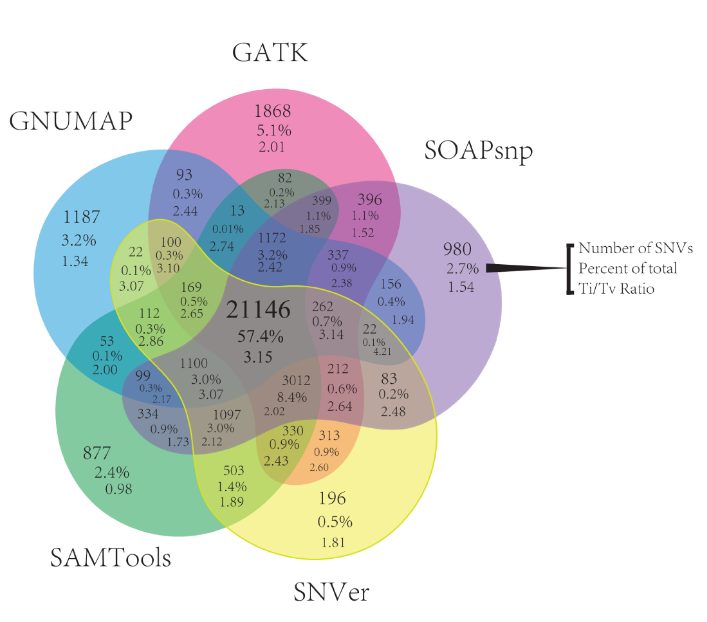
\includegraphics[width=\textwidth,height=0.8\textheight]{figs/discordance.png}
\end{frame}

\begin{frame}[fragile]{SAMtools Example}
\phantomsection\label{samtools-example}
Multiple sample SNP calling:

\begin{Shaded}
\begin{Highlighting}[]
\CommentTok{\#\# Load samtools}
\ExtensionTok{module}\NormalTok{ load samtools}

\CommentTok{\#\# mpileup}
\ExtensionTok{samtools}\NormalTok{ mpileup }\AttributeTok{{-}f}\NormalTok{ genomefile.fa }\DataTypeTok{\textbackslash{} }
  \ExtensionTok{myalignments.sorted.bam} \OperatorTok{\textgreater{}}\NormalTok{ myalignments.vcf}
\end{Highlighting}
\end{Shaded}
\end{frame}

\begin{frame}[fragile]{GATK Example}
\phantomsection\label{gatk-example}
\begin{Shaded}
\begin{Highlighting}[]
\ExtensionTok{module}\NormalTok{ load gatk}
\ExtensionTok{gatk}\NormalTok{ HaplotypeCaller }\DataTypeTok{\textbackslash{}}
    \AttributeTok{{-}R}\NormalTok{ chrX\_5MB.fa }\AttributeTok{{-}I}\NormalTok{ proband\_short\_bwa.sorted.bam }\DataTypeTok{\textbackslash{}}
    \AttributeTok{{-}O}\NormalTok{ proband\_short.vcf}
\end{Highlighting}
\end{Shaded}
\end{frame}

\begin{frame}{VCF files}
\phantomsection\label{vcf-files}
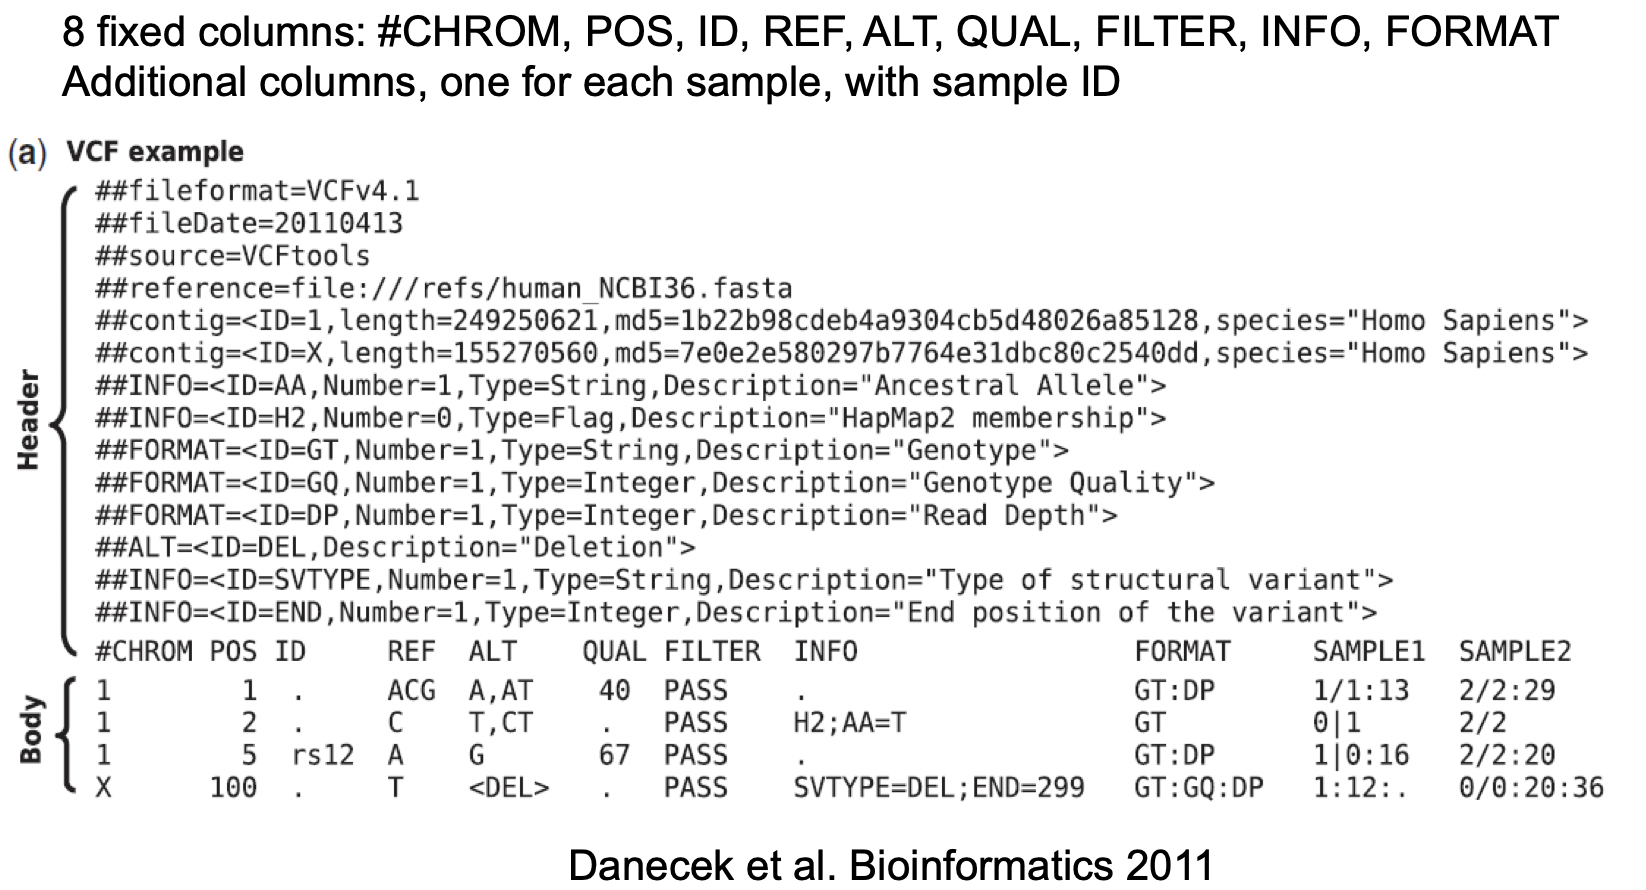
\includegraphics{figs/vcf_format.png}
\end{frame}

\begin{frame}{Complete Variant Calling Pipeline (Outdated!)}
\phantomsection\label{complete-variant-calling-pipeline-outdated}
Our analysis pipeline consisted of the following:

\begin{itemize}
\tightlist
\item
  Align the FASTQ files to genome
\item
  Convert SAM file to BAM, add read group info
\item
  Filter the reads based on quality (BAMTools)
\item
  Samtools to sort and index, and use Picard to mark duplicates
\item
  GATK calibration, realignment, variant calling (HaplotypeCaller,
  Mutect2)
\item
  Filter the called variants (GATK filtersnps and filterindels).
\item
  Annotation of SNPs (snpEff, condel)
\item
  Filter by frequency (thousand genomes, TCGA, etc.)
\item
  Downstream analysis (rare variants, pedigree, pathway level, etc)
\end{itemize}
\end{frame}

\begin{frame}{Genome Wide Association Studies (GWAS)}
\phantomsection\label{genome-wide-association-studies-gwas}
\Large

\begin{itemize}
\tightlist
\item
  Which SNPs are associated with a variable of interest?

  \begin{itemize}
  \tightlist
  \item
    e.g.~disease, height Does the frequency of any SNP differ between
    groups? Associated SNPs have:
  \end{itemize}
\item
  Effect size - e.g.~amount of increased risk
\item
  p-value - precision of effect
\item
  \textbf{Risk allele}: allele associated with increased or decreased
  probability of having a disease
\end{itemize}
\end{frame}

\begin{frame}{Genome Wide Association Studies (GWAS)}
\phantomsection\label{genome-wide-association-studies-gwas-1}
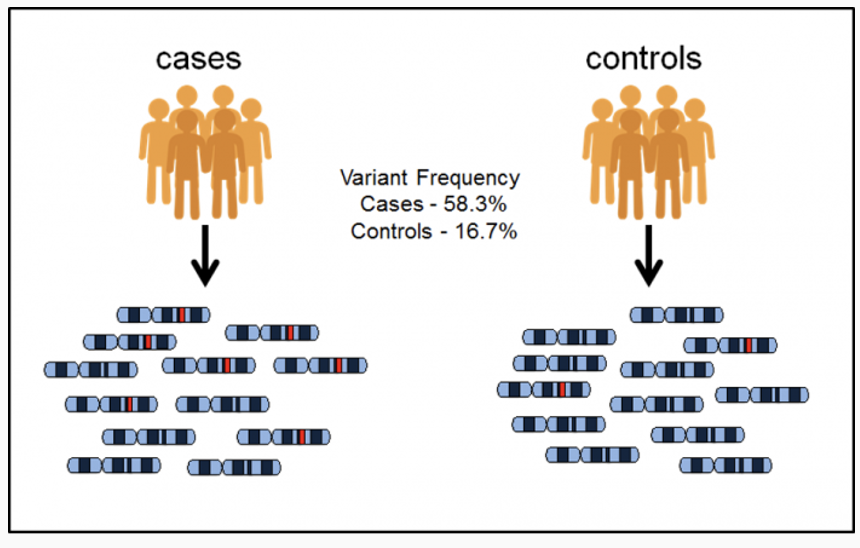
\includegraphics{figs/gwas.png}
\end{frame}

\begin{frame}{Manhattan Plot}
\phantomsection\label{manhattan-plot}
\begin{itemize}
\tightlist
\item
  In a \textbf{Manhattan plot}, each dot represents a genetic marker
  (SNP) on the x-axis, and its -log10(p-value) on the y-axis.
\item
  The horizontal lines represent the significance threshold.
\item
  Peaks represent regions where genetic variants are significantly
  associated with the trait or disease.
\end{itemize}

\center

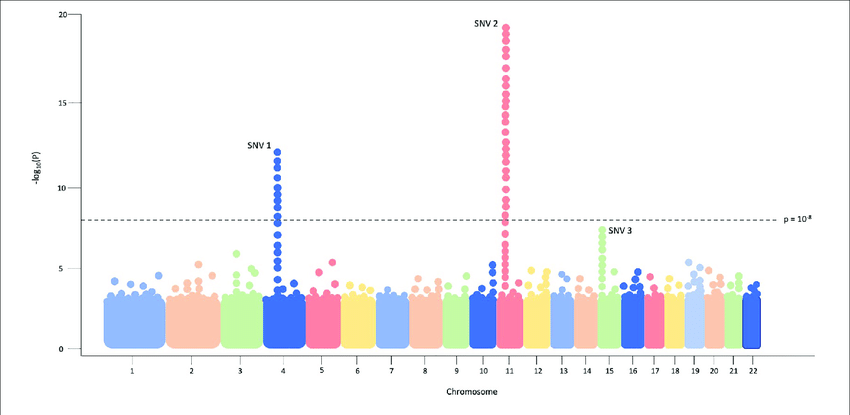
\includegraphics[width=0.8\textwidth,height=\textheight]{figs/manhattan.png}
\end{frame}

\begin{frame}{Genome-Wide Significance Threshold}
\phantomsection\label{genome-wide-significance-threshold}
\Large

\begin{itemize}
\tightlist
\item
  The genome-wide significance threshold is a threshold used to
  determine if an association between a genetic variant and a trait is
  statistically significant.
\item
  It takes into account the multiple comparisons problem arising from
  testing thousands or millions of genetic markers across the genome.
\end{itemize}
\end{frame}

\begin{frame}{Bonferroni Correction}
\phantomsection\label{bonferroni-correction}
\Large

\begin{itemize}
\tightlist
\item
  One method to establish the genome-wide significance threshold is the
  Bonferroni correction.
\item
  The Bonferroni-corrected threshold is calculated by dividing the
  desired significance level (e.g., 0.05) by the number of tests
  performed.
\item
  The most commonly accepted threshold is \[p < 5\times 10^{-8},\] based
  on a Bonferroni correction for all independent common SNPs across the
  human genome
\end{itemize}
\end{frame}

\begin{frame}{False Discovery Rate (FDR)}
\phantomsection\label{false-discovery-rate-fdr}
\Large

\begin{itemize}
\tightlist
\item
  Another method to control for multiple comparisons is the False
  Discovery Rate (FDR).
\item
  FDR controls the proportion of false positives among all significant
  results.
\item
  It is less conservative than the Bonferroni correction and allows for
  a higher number of false positives while still controlling the overall
  error rate.
\end{itemize}
\end{frame}

\begin{frame}{Downstream Annotation and Analysis (Outdated!)}
\phantomsection\label{downstream-annotation-and-analysis-outdated}
\large

Downstream Annotation Tools (old list):

\begin{itemize}
\tightlist
\item
  snpEff (\url{http://snpeff.sourceforge.net/})
\item
  Condel (\url{http://bg.upf.edu/condel/home})
\item
  SIFT \url{http://sift.jcvi.org/}
\item
  Polyphen 2 \url{http://genetics.bwh.harvard.edu/pph2/}
\item
  \url{http://mutationassessor.org/}
\item
  Ensembl variant effect predictor
  (\url{http://www.ensembl.org/info/docs/variation/vep/index.html})
\item
  Thousand Genomes variant frequency (e.g.~1\% threshold) and Exome
  Sequence Project variant frequency (e.g.~1\%).
\end{itemize}
\end{frame}

\begin{frame}[fragile]{Session info}
\phantomsection\label{session-info}
\tiny

\begin{Shaded}
\begin{Highlighting}[]
\FunctionTok{sessionInfo}\NormalTok{()}
\end{Highlighting}
\end{Shaded}

\begin{verbatim}
## R version 4.4.0 (2024-04-24)
## Platform: aarch64-apple-darwin20
## Running under: macOS Sonoma 14.2.1
## 
## Matrix products: default
## BLAS:   /Library/Frameworks/R.framework/Versions/4.4-arm64/Resources/lib/libRblas.0.dylib 
## LAPACK: /Library/Frameworks/R.framework/Versions/4.4-arm64/Resources/lib/libRlapack.dylib;  LAPACK version 3.12.0
## 
## locale:
## [1] en_US.UTF-8/en_US.UTF-8/en_US.UTF-8/C/en_US.UTF-8/en_US.UTF-8
## 
## time zone: America/Los_Angeles
## tzcode source: internal
## 
## attached base packages:
## [1] stats     graphics  grDevices utils     datasets  methods   base     
## 
## loaded via a namespace (and not attached):
##  [1] compiler_4.4.0    fastmap_1.1.1     cli_3.6.2         tools_4.4.0      
##  [5] htmltools_0.5.8.1 rstudioapi_0.16.0 yaml_2.3.8        rmarkdown_2.26   
##  [9] knitr_1.46        xfun_0.43         digest_0.6.35     rlang_1.1.3      
## [13] evaluate_0.23
\end{verbatim}
\end{frame}

\end{document}
